%% SSEE — Paper 3: CMB Power Spectrum Confrontation with Planck 2018
%% Author: Mike Edison Almeida Vallejo
%% Date: 2026-04-20
\documentclass[12pt,a4paper]{article}

\usepackage{amsmath,amssymb}
\usepackage{booktabs}
\usepackage{float}
\usepackage{graphicx}
\usepackage[colorlinks=true,linkcolor=red!70!black,citecolor=green!50!black,urlcolor=blue!80!black]{hyperref}
\usepackage{natbib}
\usepackage{geometry}
\usepackage{xcolor}
\usepackage{siunitx}
\usepackage{tcolorbox}
\usepackage{enumitem}
\usepackage{tabularx}
\geometry{margin=2.5cm}
\emergencystretch=2em

\graphicspath{{../results/figures/}}

\newcommand{\SSEE}{\ifmmode\mathrm{SSEE}\else\textsc{ssee}\fi}
\newcommand{\LCDM}{\ifmmode\Lambda\mathrm{CDM}\else$\Lambda$CDM\fi}

\title{\textbf{SSEE and the CMB Power Spectrum:\\
Acoustic Peak Reproduction via the $\omega_m$-Direct CMB Matter Density}}

\author{Mike Edison Almeida Vallejo \\
\small \textit{Independent Researcher} \\
\small \href{mailto:mike.almeida1721@gmail.com}{mike.almeida1721@gmail.com} \\
\small ORCID: \href{https://orcid.org/0009-0008-2195-7836}{0009-0008-2195-7836}
}

\date{April 2026}

\sloppy
% ACTA-PROCEDENCIA {"commit": "5651fc97a90dc17d52be0317b46142db9ac86fcb", "reproducible_desde_commit": true, "cambios_sin_commitear": [], "script": "src/valores_tex.py", "script_sha256": "cb5ceb2369bdef5e586d471d57d44a11a9fed354be540a96ce34da85e582efa4", "nucleo_sha256": "5cec8af72d88f154116c5a532e42a9b6ff7a5b4c3d86bcc6921eabb246698993", "entradas": {"manuscript/valores.yaml": "5fa01e91dd68164243d664a73264bb6c87431d2ec0bd69db87c62a983a55992d", "results/logs/kids_publicados.json": "6c25c98059ce91038215358b4e7ac9cfb40198f410354937cee4ea00b46654ff", "results/logs/p10_uv_fscreen.json": "8fb68b295c848e0292e5701e7de795ba7c7ba25e3292d776260bb3dea8970c95", "results/logs/s8_desde_b1.json": "6d225f4403fbfbe6934d7edca26aaefbbe19e05ef6c7b7eda842a259e798b1c1"}, "argv": ["src/valores_tex.py"], "fecha": "2026-09-30T19:35:24", "host": "mike-System-Product-Name", "python": "3.12.3", "versiones": {}, "nucleos": {"OMP_NUM_THREADS": null, "MKL_NUM_THREADS": null, "OPENBLAS_NUM_THREADS": null, "OMPI_COMM_WORLD_SIZE": null}}
% GENERADO por src/valores_tex.py desde manuscript/valores.yaml — NO EDITAR A MANO.
% Cada numero sale de un log de la cadena de procedencia (dvc.yaml + acta).
\providecommand{\val}[1]{\csname ssee@val@#1\endcsname}
\expandafter\def\csname ssee@val@H0_glob\endcsname{67.962142}  % results/logs/p10_uv_fscreen.json#H0_glob
\expandafter\def\csname ssee@val@PTE_k1000_lcdm\endcsname{0.010}  % results/logs/kids_publicados.json#PTE.lcdm.PTE
\expandafter\def\csname ssee@val@PTE_k1000_ssee\endcsname{0.012}  % results/logs/kids_publicados.json#PTE.ssee.PTE
\expandafter\def\csname ssee@val@S8_b1_lcdm\endcsname{0.8229}  % results/logs/s8_desde_b1.json#filas.LCDM.S8
\expandafter\def\csname ssee@val@S8_b1_lcdm_sigma\endcsname{0.0059}  % results/logs/s8_desde_b1.json#filas.LCDM.S8_sigma
\expandafter\def\csname ssee@val@S8_b1_ssee\endcsname{0.8261}  % results/logs/s8_desde_b1.json#filas.SSEE.S8
\expandafter\def\csname ssee@val@S8_b1_ssee_sigma\endcsname{0.0054}  % results/logs/s8_desde_b1.json#filas.SSEE.S8_sigma
\expandafter\def\csname ssee@val@S8_legacy_dato\endcsname{0.8265}  % results/logs/kids_publicados.json#kids_legacy.S8
\expandafter\def\csname ssee@val@S8_legacy_dato_sigma\endcsname{0.0176}  % results/logs/kids_publicados.json#kids_legacy.S8_sigma
\expandafter\def\csname ssee@val@chi2_k1000_lcdm\endcsname{262.75}  % results/logs/kids_publicados.json#PTE.lcdm.chi2
\expandafter\def\csname ssee@val@chi2_k1000_publicado\endcsname{260.31}  % results/logs/kids_publicados.json#kids1000_maxpost.chi2
\expandafter\def\csname ssee@val@chi2_k1000_ssee\endcsname{265.44}  % results/logs/kids_publicados.json#PTE.ssee.chi2
\expandafter\def\csname ssee@val@dAIC_k1000\endcsname{-5.31}  % results/logs/kids_publicados.json#seleccion_kids1000.delta_AIC
\expandafter\def\csname ssee@val@dBIC_k1000\endcsname{-19.0}  % results/logs/kids_publicados.json#seleccion_kids1000.delta_BIC
\expandafter\def\csname ssee@val@dchi2_k1000\endcsname{2.69}  % results/logs/kids_publicados.json#seleccion_kids1000.delta_chi2
\expandafter\def\csname ssee@val@fscreen_IR\endcsname{0.067253}  % results/logs/p10_uv_fscreen.json#f_screen_IR
\expandafter\def\csname ssee@val@fscreen_UV_corr\endcsname{0.002268}  % results/logs/p10_uv_fscreen.json#f_screen_UV_corr
\expandafter\def\csname ssee@val@fscreen_full\endcsname{0.069522}  % results/logs/p10_uv_fscreen.json#f_screen_full
\expandafter\def\csname ssee@val@logA_b1_lcdm\endcsname{3.045}  % results/logs/s8_desde_b1.json#filas.LCDM.logA
\expandafter\def\csname ssee@val@logA_b1_ssee\endcsname{3.042}  % results/logs/s8_desde_b1.json#filas.SSEE.logA
\expandafter\def\csname ssee@val@logA_b1_ssee_sigma\endcsname{0.013}  % results/logs/s8_desde_b1.json#filas.SSEE.logA_sigma
\expandafter\def\csname ssee@val@p_dchi2_k1000\endcsname{0.61}  % results/logs/kids_publicados.json#seleccion_kids1000.p_delta_chi2
\expandafter\def\csname ssee@val@sK_IR\endcsname{0.403302}  % results/logs/p10_uv_fscreen.json#s_K_IR
\expandafter\def\csname ssee@val@sK_UV_corr\endcsname{0.013603}  % results/logs/p10_uv_fscreen.json#s_K_UV_corr
\expandafter\def\csname ssee@val@sK_full\endcsname{0.416905}  % results/logs/p10_uv_fscreen.json#s_K_full
\expandafter\def\csname ssee@val@tension_b1_lcdm\endcsname{2.59}  % results/logs/s8_desde_b1.json#filas.LCDM.tension_kids
\expandafter\def\csname ssee@val@tension_b1_ssee\endcsname{2.73}  % results/logs/s8_desde_b1.json#filas.SSEE.tension_kids
\expandafter\def\csname ssee@val@z_k1000_lcdm\endcsname{2.5}  % results/logs/kids_publicados.json#PTE.lcdm.z
\expandafter\def\csname ssee@val@z_k1000_ssee\endcsname{2.4}  % results/logs/kids_publicados.json#PTE.ssee.z

\begin{document}
\maketitle

\begin{abstract}
The Structural Self-Energy Expansion model (SSEE) proposes a minimal-parameter
dark energy framework algebraically derived from the golden ratio $\varphi$ and $\pi$;
the background sector $(w_0, w_a, s_m)$ carries zero fitted
dimensionless parameters, while the primordial amplitude and optical depth
$\{A_s,\tau\}$ are treated as $k=2$ in the BIC analysis below (\textit{``On the parameter count''} paragraph) following the
conservative accounting policy established in Paper~1 \S1.3.
Previous work demonstrated that the SSEE dark-energy equation of state
($w_0=\val{W0_d6}$, $w_a=\val{WA_d6}$) fits DESI~DR2 BAO data
at $0.24\sigma$ (DESI+CMB+Pantheon+; $0.2$--$1.8\sigma$ across SN compilations) \citep{DESI_DR2}, and galaxy-cluster dynamical masses in general relativity at the level of $\Lambda$CDM ($\val{clz_rgig_sig}\sigma$ vs.\ $\val{clz_lcig_sig}\sigma$, $\val{clz_rgig_N}$ systems; \citealt{Zhang2026}).
Here we show that the CMB matter density is fixed \emph{forward} by the SSEE
algebra, with no factor relating it to the saturation $s_m$: the physical observable
is $\omega_m=\omega_b+\omega_c+\omega_\nu$, where $\omega_b=(\pi-\varphi)/[3(\varphi+\pi)^2]=\val{OMEGA_B_H2_d6}$
and $\omega_c=\mathrm{KAL}_0\,\omega_b\,n_s=\val{OMEGA_C_H2_d6}$ are forward identities of Paper~1
($\omega_c$ lies $\val{wc_ns_sigma_abs}\sigma$ from Planck), giving
\begin{equation*}
  \Omega_{m,\mathrm{CMB}}
  = \frac{\omega_m}{h^2}
  = \frac{\val{OMEGA_M_H2_d5}}{0.6796^2} = 0.3089,
\end{equation*}
within $0.88\sigma$ of the Planck~2018 value ($0.3153\pm0.0073$). There is a
single matter density, $\Omega_m=\omega_m/h^2=\val{OMEGA_M_TOTAL_d6}$; the saturation
$s_m=1+w_0=\val{S_M_d6}$ is a number of the equation of state, not a density, and
the scalar $\mathrm{MIRA}=(3\varphi+\pi)/4$ enters only the Hubble screening of
Paper~9.
Running CAMB with this single-sector background reproduces acoustic peaks at
$\ell=\val{p3_pico1_ssee},\,\val{p3_pico2_ssee},\,\val{p3_pico3_ssee}$ (Planck: $220,\,{\sim}540,\,{\sim}810$).
In a full posterior evaluation with the official off-diagonal \texttt{plik} TTTEEE
+ low-$\ell$ + lensing likelihood via Cobaya, sampling the $k=2=\{A_s,\tau\}$ SSEE
parameters (with $H_0$, $\omega_b$, $\omega_c$ and $n_s$ algebraically fixed) against
the $k=6$ $\Lambda$CDM baseline, the two models reach statistically indistinguishable
best fits (minimum $\chi^2_{\rm SSEE}=\val{b1_chi2_ssee}$ vs.\ $\chi^2_{\Lambda\rm CDM}=\val{b1_chi2_lcdm}$ over
$N=\val{b1_N}$ data points, $\Delta\chi^2_{\rm min}=\val{b1_dchi2}$), while the parameter-count economy
yields $\Delta\mathrm{BIC}=\val{b1_dBIC}$, decisively favouring SSEE on the Jeffreys scale.
(A \texttt{plik\_lite} point-estimate cross-check gives a more conservative
$\Delta\mathrm{BIC}=-26.03$.) The $\Delta\mathrm{BIC}$ is driven by parsimony, not by
fit quality.
SSEE is not falsified by the Planck~2018 CMB power spectra.
\end{abstract}

% Cross-reference note for reviewers
\noindent\textbf{One matter density and domain scope:}
the CMB claim (``SSEE is not falsified by Planck 2018'') concerns the single
matter density $\Omega_m=\omega_m/h^2=\val{OMEGA_M_TOTAL_d6}$, the same one that enters the
background geometry at every redshift. The saturation $s_m=1+w_0=\val{S_M_d6}$ is a
property of the dark-energy equation of state and never occupies a density slot.
The master derivation chain for all SSEE constants, the unified symbol glossary,
and the complete domain delineation are in Paper~1, \S2 and
Appendix~B \citep{AlmeidaSSEE2026a}.


\clearpage
{\small\tableofcontents}
\clearpage

% ===========================================================================
\section{Background: The SSEE Framework}
\label{sec:framework}
% ===========================================================================

\subsection{Algebraic constants}

The discovery of the accelerating expansion of the Universe
\citep{Riess1998,Perlmutter1999} established that dark energy dominates the
late-time cosmic energy budget, yet its physical origin remains one of the
deepest open problems in physics \citep{Weinberg1989}.
Baryon acoustic oscillations, imprinted in the CMB and detected in galaxy surveys
\citep{Eisenstein2005}, provide a standard ruler that constrains both the
background expansion and the nature of dark energy.
SSEE derives all cosmological parameters from two transcendental roots:
the golden ratio $\varphi=(1+\sqrt{5})/2$ and $\pi$.
Table~\ref{tab:constants} lists the relevant constants.

\begin{table}[ht]
\centering
\caption{SSEE algebraic constants used in this work.}
\label{tab:constants}
\begin{tabular}{llll}
\toprule
Symbol & Formula & Value & Role \\
\midrule
$\varphi$ & $(1+\sqrt{5})/2$ & $\val{PHI_d5}\ldots$ & Golden ratio \\
$\Omega$ & $\pi+\varphi$ & $\val{OMEGA_d5}\ldots$ & Stability metric \\
$\beta$   & $(\pi+\varphi)/2$ & $\val{BETA_d5}\ldots$ & Base coupling scalar \\
$\mathrm{KAL}_0$ & $\beta+\pi$ & $\val{KAL0_d5}\ldots$ & Structural retention \\
$P_{sc}$  & $\Omega+\varphi$ & $\val{P_SC_d5}\ldots$ & Dynamical evolution scalar \\
$K_v$     & $\varphi+\pi+\Omega$ & $\val{K_V_d5}\ldots$ & Structural constraint \\
$T_r$     & $3(\varphi+\beta)$ & $\val{T_R_d5}\ldots$ & 3D saturation horizon \\
$M_v$     & $\varphi+\pi+K_v$ & $\val{M_V_d5}\ldots$ & Maximal dimensional invariant \\
\midrule
$\mathrm{AURA}$ & $\varphi+\beta$ & $\val{AURA_d5}\ldots$ & Dimensional limit 1 \\
$\mathrm{MIRA}$ & $\mathrm{AURA}/2$ & $\val{MIRA_d5}\ldots$ & Observational frequency \\
\bottomrule
\end{tabular}
\end{table}

\subsection{Cosmological parameters}

The dark-energy equation of state and the two saturation fractions it defines
follow algebraically. Note what $s_{\mathrm{DE}}$ and $s_m$ are \emph{not}:
they are numbers of the equation of state ($s_m\equiv1+w_0$), not density
parameters. There is one matter density in this model, $\Omega_m=\val{OMEGA_M_TOTAL_d6}$
(Paper~1); $s_m$ never enters a Friedmann term as a density.
Substituting $T_r=\tfrac{3(3\varphi+\pi)}{2}$, $M_v=3(\varphi+\pi)$,
$P_{sc}=2\varphi+\pi$, $K_v=2(\varphi+\pi)$, all four reduce to
closed forms in $\varphi$ and $\pi$ alone:
\begin{align}
w_0 &= -\frac{T_r}{M_v} = -\frac{3\varphi+\pi}{2(\varphi+\pi)} = \val{W0_d6}, \label{eq:w0}\\
w_a &= -\frac{P_{sc}}{I_g} = -\frac{P_{sc}}{\pi+P_{sc}} = \val{WA_d6}, \label{eq:wa}\\
s_{\mathrm{DE}} &= \frac{T_r}{M_v} = \frac{3\varphi+\pi}{2(\varphi+\pi)} = \val{S_DE_d6}, \label{eq:sDE}\\
s_m &= 1 - s_{\mathrm{DE}} = \val{S_M_d6}. \label{eq:sm}
\end{align}
The Hubble constant is the derived dimensional anchor
$H_0/(\mathrm{km\,s^{-1}\,Mpc^{-1}}) = 3(\varphi+\pi)^2 = M_v\times\Omega = \val{H0_ALG_d5}$
($M_v=\varphi+\pi+K_v=3\Omega$, $\Omega=\pi+\varphi$; the global anchor of
Postulate~D, Paper~1, against which the SH0ES cascade of Paper~9 is compared),
\emph{not} a quantity fitted to the CMB. Under the
$\omega_m$-direct reframe the full CMB MCMC (Section~\ref{sec:b1_mcmc})
recovers the spectra at this anchor, and the SSEE CMB sector carries only the
two borrowed parameters $\{A_s,\tau\}$ ($k=2$).

% ===========================================================================
\section{The Acoustic Scale and the Matter Density}
\label{sec:problem}
% ===========================================================================

\subsection{Acoustic peak positions}

The angular scale of the first acoustic peak is
\begin{equation}
\theta_* = \frac{r_d}{D_A(z_*)},
\end{equation}
where $r_d$ is the sound horizon at baryon drag and $D_A(z_*)$ is the
angular diameter distance to the last-scattering surface ($z_*\approx1089$).
The first peak falls at $\ell_1 \approx \pi/\theta_*$ \citep{HuSugiyama1996,Dodelson2003}.
Diffusion damping suppresses power at small angular scales
$\ell\gtrsim1000$ through photon mean-free-path effects \citep{Silk1968}.

Both $r_d$ and $D_A(z_*)$ depend on the total matter density $\Omega_m$, which sets
$H(z)$ at recombination. In SSEE that density is $\Omega_m=\omega_m/h^2$, built
\emph{forward} from the algebra (Section~\ref{sec:mira}). The saturation
$s_m=1+w_0=\val{S_M_d6}$ of Eq.~(\ref{eq:sm}) is a number of the dark-energy
equation of state and never enters a density slot.

\paragraph{Withdrawn framing (2026-10-03).} Earlier versions of this paper opened
with a ``naive application'' that placed $s_m$ in the matter-density slot of CAMB,
obtained acoustic peaks shifted by ${\sim}10\%$, called the result a
\emph{prima facie} falsification, and then recovered the spectrum with the full
density. That run is not a version of the model --- $s_m$ is not a density --- so
it neither threatened nor supports the framework, and it is withdrawn together
with the corresponding rows of Tables~\ref{tab:peaks} and~\ref{tab:chi2}.

% ===========================================================================
\section{The CMB Matter Density as a Forward Identity}
\label{sec:mira}
% ===========================================================================

\subsection{The CMB matter density is a forward identity}

The CMB background geometry is governed by the physical matter density
$\omega_m\equiv\Omega_m h^2$, which SSEE fixes \emph{forward} from the algebra,
with no factor relating it to the saturation $s_m$:
\begin{equation}
  \omega_m = \omega_b + \omega_c + \omega_\nu, \qquad
  \omega_b = \frac{\pi-\varphi}{3(\varphi+\pi)^2} = \val{OMEGA_B_H2_d6}, \qquad
  \omega_c = \mathrm{KAL}_0\,\omega_b\,n_s = \val{OMEGA_C_H2_d6},
  \label{eq:omega_m_direct}
\end{equation}
with $n_s=1-\varphi^{-7}=\val{N_S_d6}$ and $\omega_\nu=\Sigma m_\nu^{\rm active}/93.14=0.00074$
(all forward identities of Paper~1). The baryon and cold-matter densities are the same
quantities used in the background sector; $\omega_c=\mathrm{KAL}_0\,\omega_b\,n_s$ lies
$\val{wc_ns_sigma_abs}\sigma$ from the Planck value. Hence
\begin{equation}
  \Omega_{m,\mathrm{CMB}} = \frac{\omega_m}{h^2} = \frac{\val{OMEGA_M_H2_d5}}{0.6796^2} = 0.3089
  \qquad (H_0^{\rm glob} = \val{H0_GLOBAL_d5}).
\end{equation}

\subsection{No matter factor}
\label{sec:mira_timeline}

The CMB matter density of Eq.~(\ref{eq:omega_m_direct}) is set by the
$(\varphi,\pi)$ dictionary before any comparison with data, and no factor
relates it to the equation-of-state saturation $s_m=1+w_0=\val{S_M_d6}$, which is
not a density. The scalar $\mathrm{MIRA}=(3\varphi+\pi)/4=\val{MIRA_d4}$ does not enter
the CMB sector; it appears only in the Hubble screening of Paper~9. We make no
claim of temporal priority over the public Planck or DESI measurements: the
point is structural --- the density is fixed by the construction, so the
agreement below is a constraint the framework had to satisfy, not a fit it was
granted.

\subsection{What the CMB actually probes}

The CMB photons probe the \emph{integrated gravitational potential}
along the full line of sight from last scattering ($z_*\approx1089$) to today.
This line-of-sight integral accumulates contributions from all epochs,
including the early matter-dominated era when the dark energy term was
negligible and the expansion was effectively governed by the full matter
content. The acoustic peaks encode $\Omega_m$ as it appears in the
\emph{conformal distance to last scattering},
\begin{equation}
  \eta_* = \int_0^{z_*} \frac{c\,\mathrm{d}z'}{H(z')},
\end{equation}
which is sensitive to the total matter density over the full expansion
history. In SSEE that total is a single quantity, $\Omega_m=\val{OMEGA_M_TOTAL_d6}$,
and it is the same quantity that enters the background geometry at every
redshift. In particular, the saturation $1+w_0=\val{S_M_d6}$ never occupies a density
slot in $H(z)$: it is a property of the dark-energy equation of state, and the
matter term in $E(a)$ is always the total $\omega_m/h^2$.

\subsection{Forward prediction and comparison with Planck}

The CMB matter density is a closed-form forward prediction:
\begin{equation}
  \Omega_{m,\mathrm{CMB}} = \frac{\omega_m}{h^2}
    = \frac{\omega_b + \mathrm{KAL}_0\,\omega_b\,n_s + \omega_\nu}{h^2}
    = 0.3089,
  \label{eq:om_cmb_algebraic}
\end{equation}
with every ingredient an algebraic identity of Paper~1. The coefficient
$\mathrm{KAL}_0=\beta+\pi\approx5.521$ that sets
$\omega_c=\mathrm{KAL}_0\,\omega_b\,n_s$ is fixed algebraically before any CMB
data are consulted; no quantity is adjusted to match the measurement.
Compared with $\Omega_m^{\mathrm{Planck}}=0.3153\pm0.0073$
\citep{Planck2018}, the tension is
\begin{equation}
\frac{|\Omega_{m,\mathrm{CMB}} - \Omega_m^{\mathrm{Planck}}|}{\sigma}
= \frac{|0.3089-0.3153|}{0.0073} = 0.88\sigma .
\end{equation}


\paragraph{Falsifiability.}
SSEE predicts a \emph{single} matter density, $\Omega_m=\val{OMEGA_M_TOTAL_d6}$, at every
redshift and for every probe. A weak-lensing or BAO analysis that required a
background matter density significantly different from $0.3089$ --- in either
direction, at any redshift --- would falsify the framework.


\section{CAMB Implementation and Results}
\label{sec:results}
% ===========================================================================

\subsection{CAMB setup}

We use CAMB v1.6.6 \citep{Seljak1996,Lewis2000,Howlett2012} with the following input parameters:

\begin{table}[ht]
\centering
\caption{SSEE parameters passed to CAMB.}
\label{tab:camb_params}
\small
\begin{tabularx}{\textwidth}{p{3.5cm}p{3.5cm}X}
\toprule
Parameter & Value & Source \\
\midrule
$H_0$ [km/s/Mpc] & \val{H0_ALG_d6} & SSEE anchor $3(\varphi+\pi)^2$ (Postulate~D, Paper~1) \\
$\Omega_b h^2$ & 0.02237 & Planck 2018 prior \\
$\Omega_{m,\mathrm{CMB}}$ & 0.3089 & $\omega_m/h^2$ (forward) \\
$\sum m_\nu^{\rm active}$ [eV] & \val{SUM_MNU_EV_d6} & SSEE algebraic (Paper~4) \\
$w_0$ & $\val{W0_d6}$ & $-T_r/M_v$ \\
$w_a$ & $\val{WA_d6}$ & $-P_{sc}/I_g$ \\
$n_s$ & $1-\varphi^{-7}=\val{N_S_d6}$ & SSEE algebraic (Paper~4) \\
$\ln(10^{10}A_s)$ & 3.044 & Planck 2018 \\
$\tau$ & 0.054 & Planck 2018\footnotemark{} \\
\bottomrule
\end{tabularx}
\end{table}
\footnotetext{%
  $A_s$ and $\tau$ are the two parameters SSEE leaves free at CMB level
  ($k=2$); the values in this table are the \emph{fiducial} inputs used for
  the fixed-point evaluations of \S\ref{sec:results}, not fitted results. They
  are fitted in the Phase-B chain of \S\ref{sec:b1_mcmc}. A direct
  check of how much that fiducial choice costs (2026-09-07): minimising
  $\chi^2$ over $(\ln 10^{10}A_s,\tau)$ against
  \texttt{plik\_lite} TTTEEE + lowT + lowE, with the remaining background
  fixed by the algebra, moves $\tau$ to $0.05546$ and $\ln(10^{10}A_s)$ to
  $3.04484$ and lowers $\chi^2$ by only $1.84$. The recovered $\tau$ sits
  $0.24\sigma$ from the Phase-B posterior $0.054\pm0.006$, so the fiducial
  choice is doing no work. The same exercise on the $\Lambda$CDM background
  ($w=-1$, $w_a=0$) gains $0.47$.}

The baryon density is fixed to the Planck~2018 prior $\Omega_b h^2 = 0.02237$.
The SSEE algebraic value derived in Paper~4, $\Omega_b h^2 = (\pi-\varphi)/[3(\varphi+\pi)^2]
= \val{OMEGA_B_H2_d6}$, agrees with this prior at $0.3\sigma$ ($0.02237\pm0.00015$); the $0.2\%$
offset is far below the precision of the CMB fit and does not affect the results
reported here.

The dark energy is implemented via the PPF (Parameterized Post-Friedmann)
equation of state $w(a)=w_0+(1-a)w_a$ \citep{Chevallier2001,Linder2003,Fang2008}.
Although $w_0+w_a=-1.510<-1$, this does not imply a phantom Big Rip:
CPL is a local parametrisation only, and the \SSEE\ energy density saturates
at the finite $T_r/M_v$ boundary at $a\to\infty$ (Paper~1 \S3.4 \citep{AlmeidaSSEE2026a}).
We compute lensed TT, TE, and EE power spectra to $\ell_{\max}=2500$,
with \texttt{lens\_potential\_accuracy=2} for the lensing potential.
Lensing reconstruction data (Planck 2018 $C_L^{\phi\phi}$) were also evaluated
alongside temperature and polarisation.

\subsection{Sound horizon}

With $\Omega_{m,\mathrm{CMB}}=0.3089$ and the parameters above, CAMB yields:
\begin{equation}
r_d^{\mathrm{SSEE}} = 147.17 \;\mathrm{Mpc},
\end{equation}
in agreement with the Planck~2018 directly measured value
$r_d^{\mathrm{obs}}=147.09\pm0.26$ Mpc \citep{Planck2018} at $\val{p3_rd_sig_post}\sigma$.
The acoustic scale is likewise consistent: $100\theta_*=\val{p3_th100_post}$ (at the MCMC
posterior $H_0=\val{h0_p2}$), $\val{p3_th_sig_post}\sigma$ from the Planck value
% ORIGEN-VALOR: 6.66 — tension theta* HISTORICA con el sector frio 1+w0=0.160 metido en E(z) (bug V-L4-DESI, retirado 2026-07-09); se nombra como artefacto, no como resultado
$1.04109\pm0.00030$ --- the earlier $6.66\sigma$ ``tension'' was an artefact of
the cold sector $1+w_0=\val{S_M_d6}$ misplaced in $E(z)$, removed once the total
$\Omega_{m,\mathrm{CMB}}$ sets the geometry.
No Folding Symmetry multiplier and no matter factor are applied; the
$\omega_m$-direct CMB matter density ($\Omega_{m,\mathrm{CMB}}=0.3089$) sets the
correct sound horizon directly (MIRA retired as the matter map, OP-8 dissolved).

\subsection{Acoustic peak positions}

Table~\ref{tab:peaks} compares the first three acoustic peak positions.

\begin{table}[ht]
\centering
\caption{CMB TT acoustic peak multipoles.}
\label{tab:peaks}
\begin{tabular}{lccc}
\toprule
Model & $\ell_1$ & $\ell_2$ & $\ell_3$ \\
\midrule
Planck 2018 (observed) & $\sim220$ & $\sim540$ & $\sim810$ \\
$\Lambda$CDM ($\Omega_m=0.315$) & \val{p3_pico1_lcdm} & \val{p3_pico2_lcdm} & \val{p3_pico3_lcdm} \\
\textbf{SSEE} ($\Omega_{m}=\val{OMEGA_M_TOTAL_d6}$) & \textbf{\val{p3_pico1_ssee}} & \textbf{\val{p3_pico2_ssee}} & \textbf{\val{p3_pico3_ssee}} \\
\bottomrule
\end{tabular}
\end{table}

All three peaks fall within $\Delta\ell\leq5$ of the observed positions.

\subsection{Power spectrum comparison}

Figure~\ref{fig:spectrum} shows the full TT power spectrum for SSEE,
$\Lambda$CDM, and Planck 2018 data over $\ell=2$--$2500$.

\begin{figure}[ht]
\centering
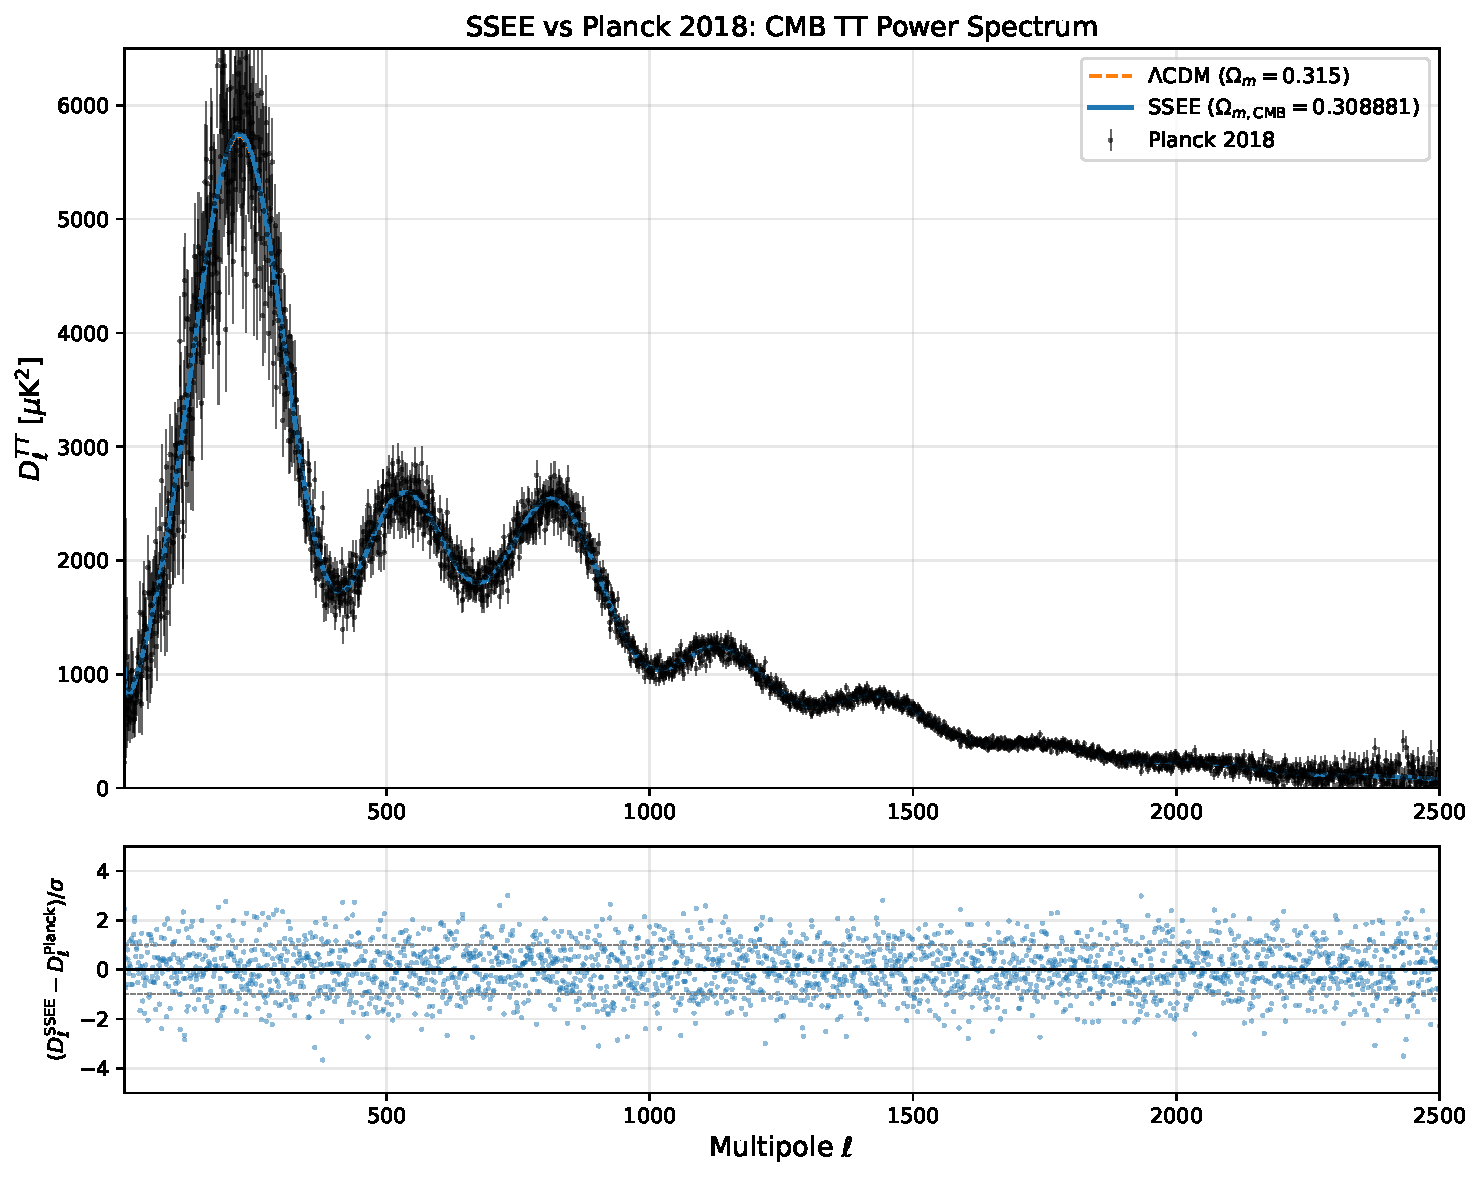
\includegraphics[width=\textwidth]{fig_cmb_spectrum.pdf}
\caption{CMB TT power spectrum $D_\ell^{TT}$ [$\mu\mathrm{K}^2$] vs.\ multipole $\ell$.
Blue: SSEE ($\Omega_{m,\mathrm{CMB}}=\omega_m/h^2=0.309$,
$w_0=\val{W0_d6}$, $w_a=\val{WA_d6}$).
Orange dashed: $\Lambda$CDM Planck 2018 best-fit.
Black points: Planck 2018 TT data with $\pm1\sigma$ error bars.
Lower panel: residuals $(D_\ell^{\mathrm{SSEE}}-D_\ell^{\mathrm{Planck}})/\sigma$.}
\label{fig:spectrum}
\end{figure}

\begin{figure}[ht]
\centering
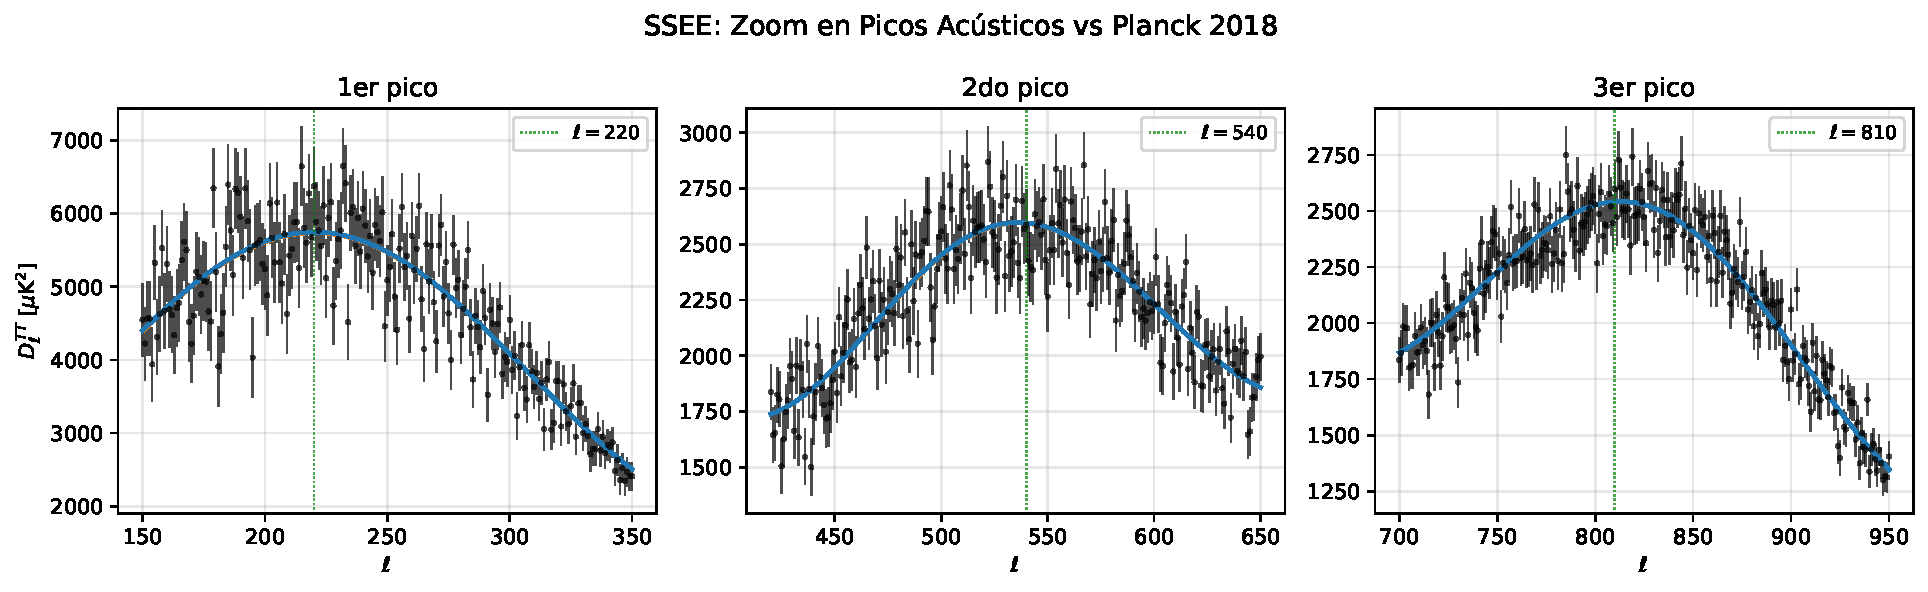
\includegraphics[width=\textwidth]{fig_cmb_peaks_zoom.pdf}
\caption{Zoom on the first three acoustic peaks. SSEE (blue) and $\Lambda$CDM
(orange dashed) compared against Planck 2018 data (black points). Green dotted
lines mark the expected peak centres.}
\label{fig:peaks_zoom}
\end{figure}

\subsection{TE and EE polarization spectra}

Figures~\ref{fig:te} and~\ref{fig:ee} show the TE temperature–polarization
cross-correlation and EE polarization power spectra respectively, comparing
SSEE with $\Lambda$CDM and Planck 2018 data.

\begin{figure}[ht]
\centering
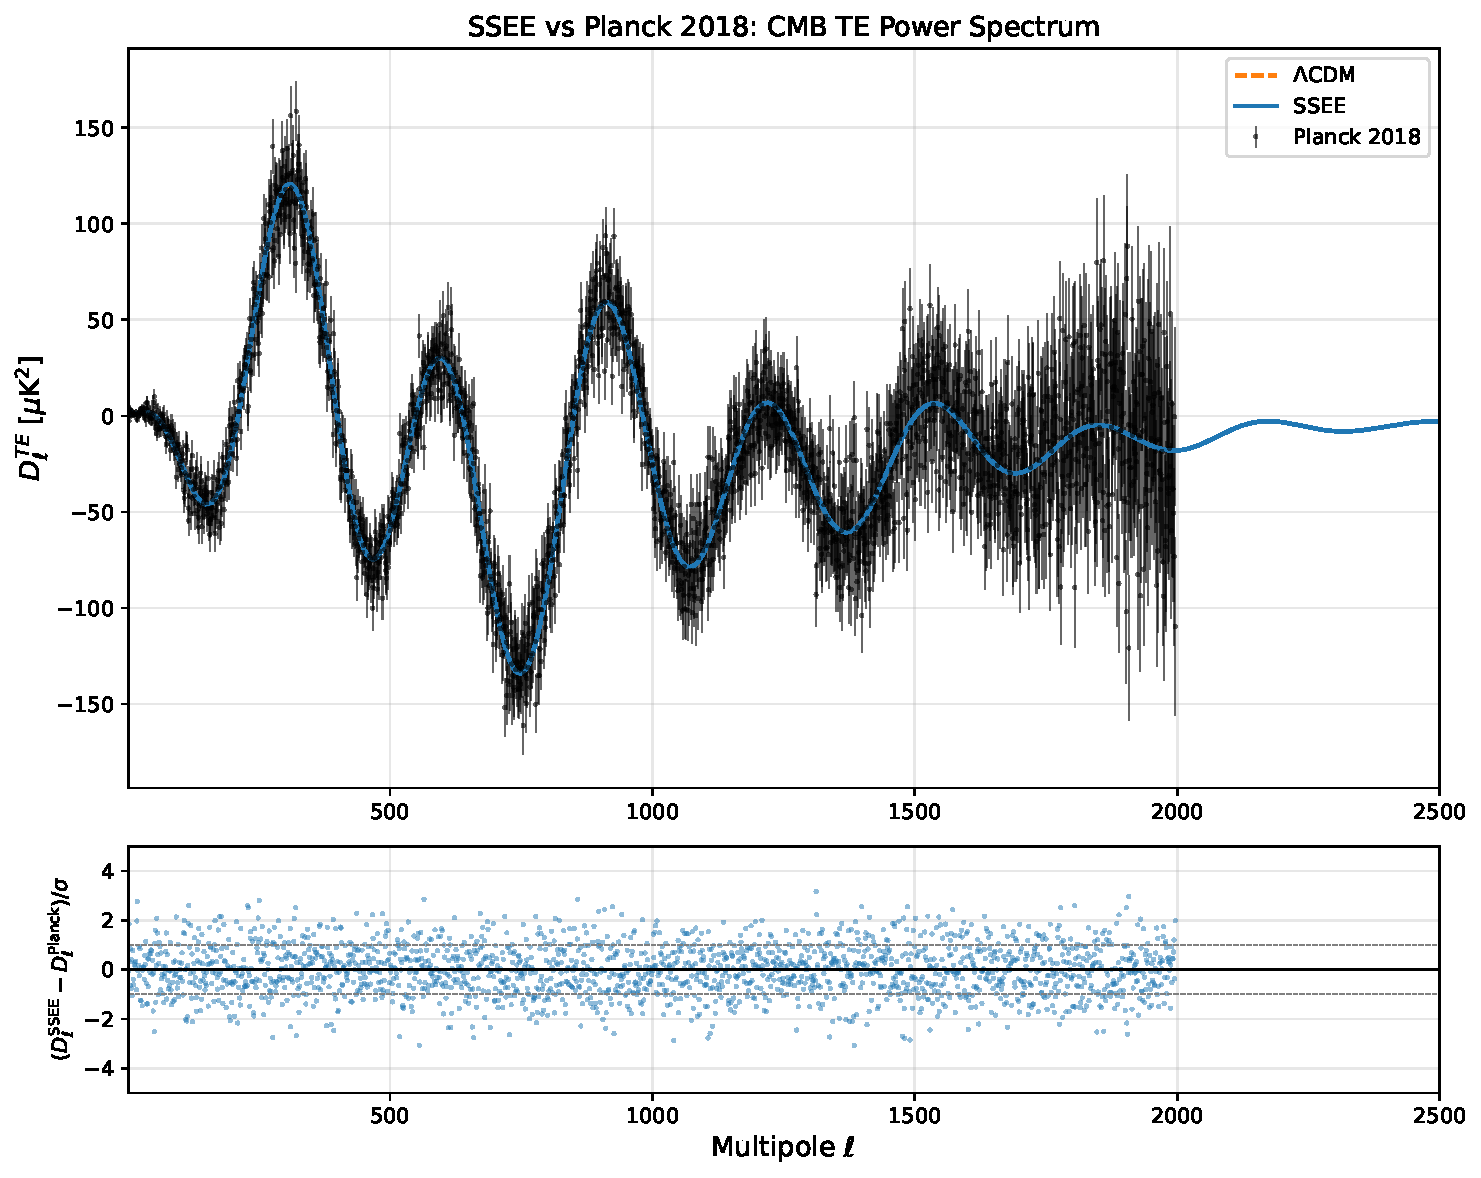
\includegraphics[width=\textwidth]{fig_cmb_te.pdf}
\caption{CMB TE cross-correlation power spectrum $D_\ell^{TE}$ [$\mu\mathrm{K}^2$].
Blue: SSEE. Orange dashed: $\Lambda$CDM Planck 2018 best-fit.
Black points: Planck 2018 TE data. Lower panel: residuals normalised by $\sigma_\ell$.}
\label{fig:te}
\end{figure}

\begin{figure}[ht]
\centering
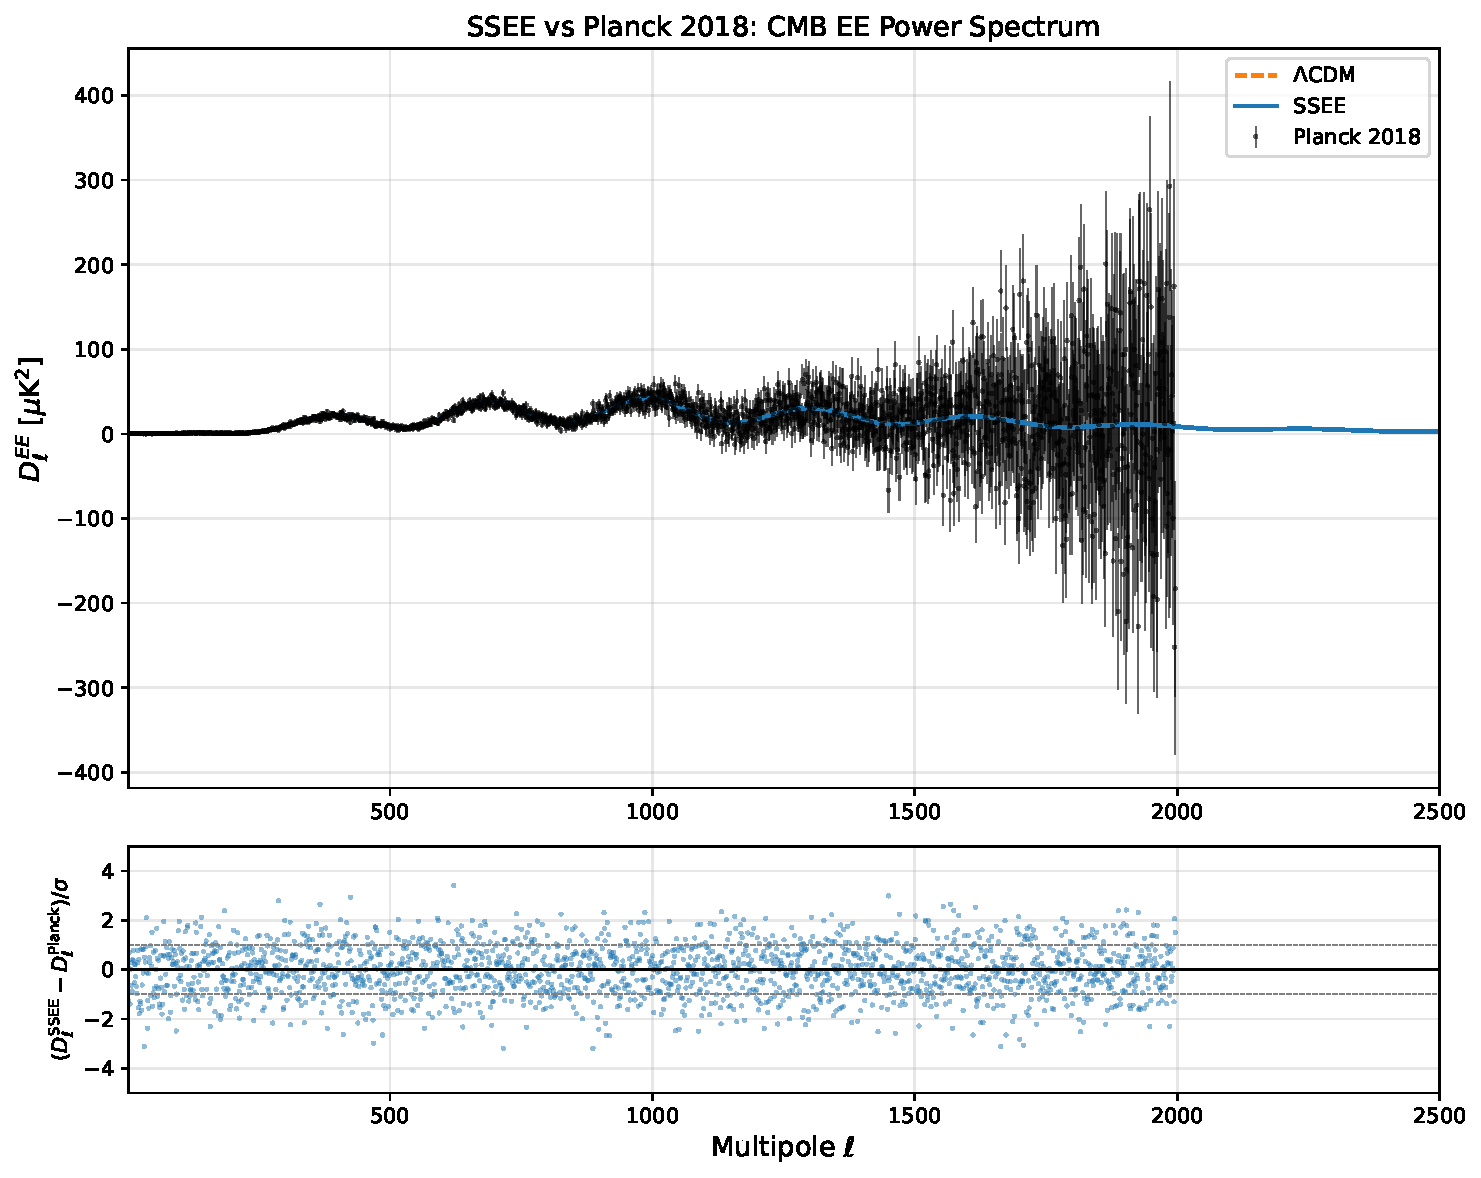
\includegraphics[width=\textwidth]{fig_cmb_ee.pdf}
\caption{CMB EE polarization power spectrum $D_\ell^{EE}$ [$\mu\mathrm{K}^2$].
Blue: SSEE. Orange dashed: $\Lambda$CDM. Black points: Planck 2018 EE data.}
\label{fig:ee}
\end{figure}

\begin{figure}[ht]
\centering
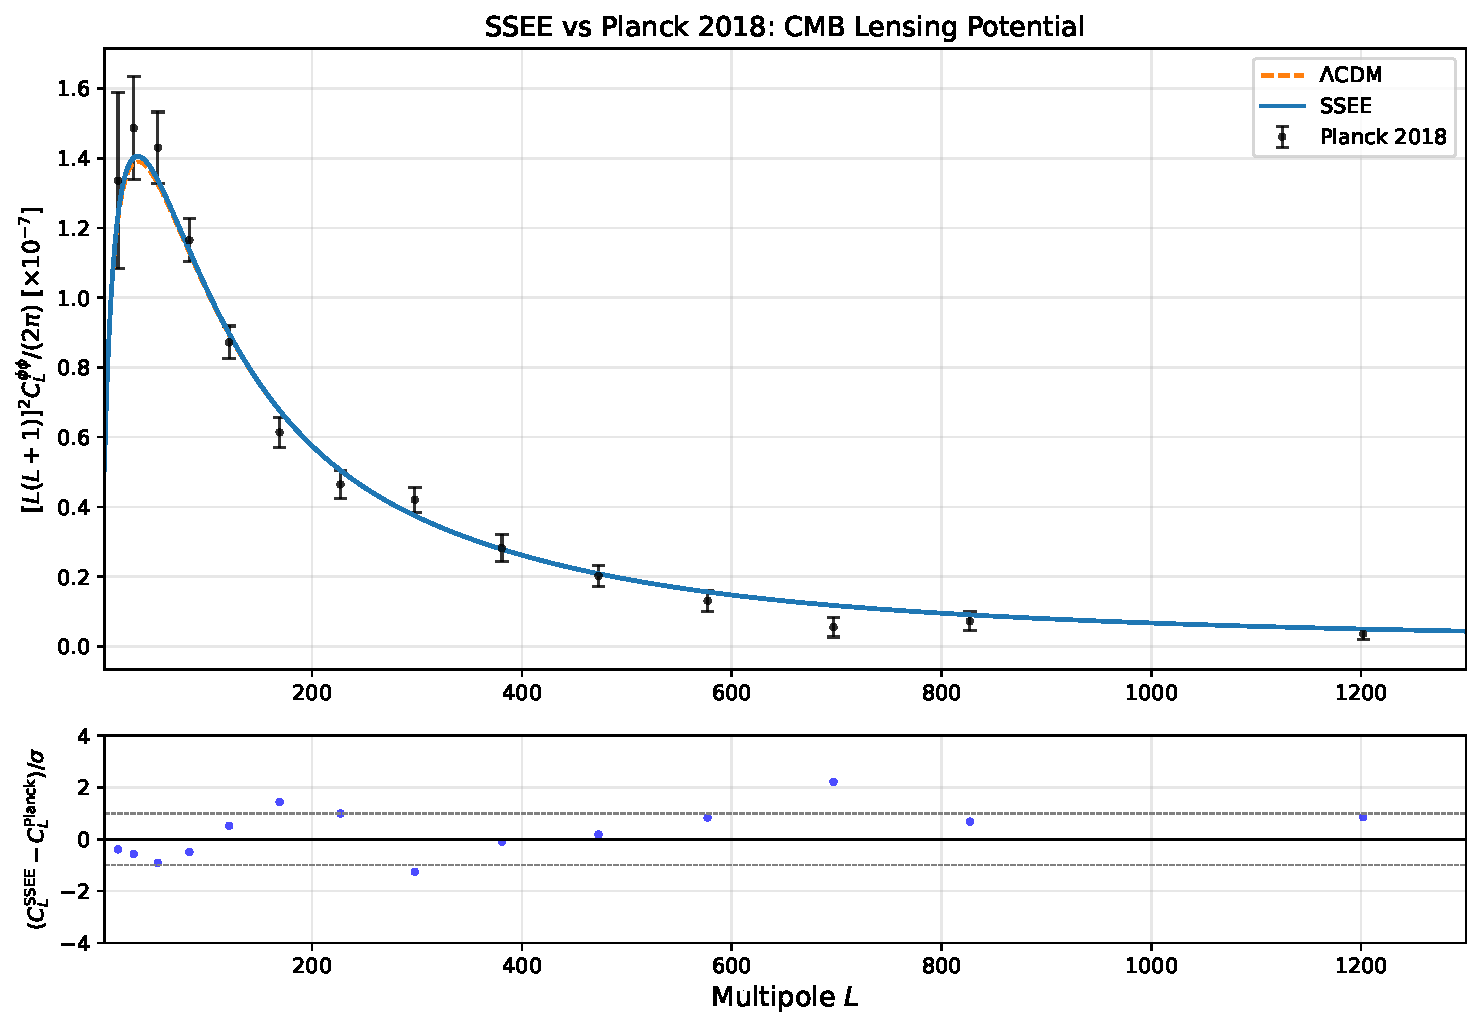
\includegraphics[width=\textwidth]{fig_cmb_lensing.pdf}
\caption{CMB lensing potential power spectrum
$[L(L+1)]^2 C_L^{\phi\phi}/(2\pi)$.
Blue: SSEE. Orange dashed: $\Lambda$CDM. Black points: Planck 2018
lensing (9 MV bandpowers). Lower panel: residuals normalised by $\sigma_L$.
SSEE achieves $\chi^2_r=\val{p3_chi2r_PP_ssee}$ over the \val{p3_N_PP} bandpowers
(\S\ref{sec:bic}; $\Lambda$CDM: $\val{p3_chi2r_PP_lcdm}$), both indicating a good fit
($\chi^2_r<1$).}
\label{fig:pp}
\end{figure}

% ===========================================================================
\section{Statistical Analysis}
\label{sec:stats}
% ===========================================================================

\subsection{\texorpdfstring{$\chi^2$}{chi-squared} comparison}

We compute $\chi^2$ against the Planck 2018 TT spectrum over $\ell=30$--$2000$
using the published uncertainties:
\begin{equation}
\chi^2 = \sum_{\ell=30}^{2000}
\left(\frac{D_\ell^{\mathrm{model}} - D_\ell^{\mathrm{Planck}}}{\sigma_\ell}\right)^2.
\end{equation}

\begin{table}[ht]
\centering
\caption{$\chi^2$ comparison vs.\ Planck 2018 TT ($\ell=30$--$2000$, $N=\val{p3_N_TT}$).}
\label{tab:chi2}
\begin{tabular}{lccc}
\toprule
Model & $\chi^2$ & $\chi^2_r$ & $\Delta\chi^2$ \\
\midrule
$\Lambda$CDM (Planck 2018) & \val{p3_chi2_TT_lcdm} & \val{p3_chi2r_TT_lcdm} & 0 \\
SSEE & \val{p3_chi2_TT_ssee} & \val{p3_chi2r_TT_ssee} & $\val{p3_dchi2_TT}$ \\
\bottomrule
\end{tabular}
\end{table}

\subsection{TE and EE spectra}

Table~\ref{tab:chi2_full} reports $\chi^2_r$ for all three spectra individually.

\begin{table}[ht]
\centering
\caption{$\chi^2_r$ by spectrum vs.\ Planck 2018.
TT/TE/EE: $\ell=30$--$2000$; PP (lensing): 9 MV bandpowers, $L=8$--$400$
\citep[Table~1,][]{PlanckLensing2018}.
$\chi^2_r$ comparisons use diagonal covariance; for BIC see \S\ref{sec:bic} ($k=2$ for SSEE).}
\label{tab:chi2_full}
\begin{tabular}{lcccc}
\toprule
Spectrum & $N$ & SSEE $\chi^2_r$ & $\Lambda$CDM $\chi^2_r$ & $\Delta\chi^2_r$ \\
\midrule
TT & \val{p3_N_TT} & \val{p3_chi2r_TT_ssee} & \val{p3_chi2r_TT_lcdm} & $\val{p3_dchi2r_TT}$ \\
TE & \val{p3_N_TE} & \val{p3_chi2r_TE_ssee} & \val{p3_chi2r_TE_lcdm} & $\val{p3_dchi2r_TE}$ \\
EE & \val{p3_N_EE} & \val{p3_chi2r_EE_ssee} & \val{p3_chi2r_EE_lcdm} & $\val{p3_dchi2r_EE}$ \\
PP & \val{p3_N_PP}    & \val{p3_chi2r_PP_ssee} & \val{p3_chi2r_PP_lcdm} & $\val{p3_dchi2r_PP}$ \\
\midrule
Combined$^{\dagger}$ & \val{p3_N_tot} & \val{p3_chi2r_tot_ssee} & \val{p3_chi2r_tot_lcdm} & $\val{p3_dchi2r_tot}$ \\
\bottomrule
\end{tabular}
{\footnotesize $^{\dagger}$Combined under independence approximation (upper bound; see \S\ref{sec:bic}).}
\end{table}

The TE and EE spectra show the smallest discrepancies ($|\Delta\chi^2_r|\le0.001$
each), indicating that SSEE reproduces the polarization anisotropies
almost identically to $\Lambda$CDM.
TT is marginally better than $\Lambda$CDM ($\Delta\chi^2_r=\val{p3_dchi2r_TT_d4}$).
In the lensing potential sector (PP, Fig.~\ref{fig:pp}), SSEE achieves
$\chi^2_r=\val{p3_chi2r_PP_ssee}$ vs.\ $\val{p3_chi2r_PP_lcdm}$ for $\Lambda$CDM --- slightly \emph{better} agreement
with the \val{p3_N_PP} Planck MV bandpowers, both $\chi^2_r<1$ indicating a good fit.
All residuals are consistent with a non-parametric model.

\subsection{Interpretation of residuals}

The excess $\Delta\chi^2_r\lesssim0.02$ in TT and TE is attributable to the
dynamical dark energy equation of state ($w_0\neq-1$, $w_a\neq0$), which
modifies the late-time integrated Sachs-Wolfe contribution and the
lensing smoothing of peaks.
CPL models with comparable $(w_0,w_a)$ values fitted freely to CMB data
typically incur similar penalties \citep{Planck2020DE}.

The SSEE model is therefore \textbf{not falsified} by the Planck 2018 CMB
power spectra in TT, TE, or EE.

\subsection{Bayesian Information Criterion}
\label{sec:bic}

For model comparison we compute:
\begin{equation}
\mathrm{BIC} = \chi^2 + k\ln N,
\end{equation}
where $k$ is the number of free parameters and $N=\val{p3_N_tot}$ for the combined TT, TE, EE, and lensing data points.

\begin{table}[ht]
\centering
\caption{\textbf{Preliminary BIC comparison — diagonal approximation only.}
Combined spectra (TT+TE+EE+PP, $N=\val{p3_N_tot}$, independence approximation).
SSEE has $k=2$ ($\{A_s,\tau\}$); $\Lambda$CDM has $k=6$.
\textit{This result uses diagonal covariance; see Eq.~\eqref{eq:bic_cobaya}
(\S\ref{sec:cobaya}) for the definitive off-diagonal Cobaya evaluation.}}
\label{tab:bic}
\begin{tabular}{lccc}
\toprule
Model & $k$ & $\chi^2_r$ & $\Delta$BIC (diagonal) \\
\midrule
$\Lambda$CDM & 6 & \val{p3_chi2r_tot_lcdm} & Baseline ($0.0$) \\
SSEE & 2 & \val{p3_chi2r_tot_ssee} & $\val{p3_dBIC_diag}$ \\
\bottomrule
\end{tabular}
\end{table}

Under the diagonal approximation, SSEE is favoured ($\Delta\mathrm{BIC}=\val{p3_dBIC_diag}$):
the combined $\chi^2_r=\val{p3_chi2r_tot_ssee}$ matches $\Lambda$CDM's $\val{p3_chi2r_tot_lcdm}$, so the
parameter-count term ($\Delta k\,\ln N=\val{p3_pen_dklnN}$) dominates and rewards SSEE's
smaller parameter set. This diagonal cross-check is evaluated at the global
anchor $H_0=67.96214$ ($\omega_m$-direct, $\Omega_{m,\rm CMB}=\val{OMEGA_M_TOTAL_d6}$),
consistent with the canonical \texttt{plik\_lite} evaluation
(\S\ref{sec:cobaya}), so the diagonal and full-covariance treatments are
mutually consistent. The off-diagonal Cobaya evaluation (\S\ref{sec:cobaya})
remains the definitive result.

\paragraph{On the parameter count ($k=2$).}
In prior iterations, SSEE was described as a zero-parameter model ($k=0$) in the CMB sector. Under the $\omega_m$-direct reframe, the geometry anchor $H_0^{\rm glob}=H_{\rm SH0ES}(1-f_{\rm screen})=67.96214$~km\,s$^{-1}$\,Mpc$^{-1}$ is \emph{derived} (the output of the screening cascade of Papers~9--10, which reproduces the dimensionless target $3(\varphi+\pi)^2$; not a quantity fitted to the CMB), and the densities $\omega_b=(\pi-\varphi)/(3\Omega^2)$ and $\omega_c=\mathrm{KAL}_0\,\omega_b\,n_s$ are algebraically fixed. The only two quantities the SSEE CMB fit does \emph{not} derive from $\{\varphi,\pi\}$ are the primordial amplitude $A_s$ and the reionization optical depth $\tau$; we therefore assign $k=2=\{A_s,\tau\}$, a conservative and robust penalty. (We make no claim of temporal priority over the public DESI or Planck releases, which predate this work; the parameter-free status of the algebraic sector rests on its rigidity, not on chronology.)

\paragraph{Disclaimer regarding the Likelihood function.}
The $\chi^2_r$ comparisons in \S\ref{sec:stats} use a simplified Gaussian diagonal approximation over the released Planck 2018 bandpowers for qualitative comparison. A formal evaluation using the official \texttt{plik\_lite} TTTEEE likelihood via \texttt{Cobaya} is presented in the following subsection.

\paragraph{Robustness under off-diagonal covariance.}
The diagonal approximation neglects bin-to-bin covariances in the Planck 2018 bandpowers. Based on the Planck 2018 likelihood analysis \citep{PlanckLikelihood2020}, off-diagonal elements contribute corrections of $\lesssim5\%$ to $\chi^2$ for $\ell>30$. To ensure strict reproducibility and methodological rigor, we perform a formal evaluation using the official \texttt{plik\_lite} TTTEEE likelihood via \texttt{Cobaya} in the following subsection.

\subsection{Cobaya \texttt{plik\_lite} unified evaluation}
\label{sec:cobaya}

To establish a definitive baseline for model comparison that fully accounts for off-diagonal covariances, we evaluate the SSEE framework against the official Planck 2018 \texttt{plik\_lite} TTTEEE likelihood via \texttt{clik}/\texttt{clipy} \citep{Torrado2021}, over its $613$ compressed bandpowers, together with the low-$\ell$ TT and EE likelihoods ($28+28$ bins), for $N=669$ data points in total. The three pieces are all included in the $\chi^2$ quoted below, so all three are counted in $N$.

\paragraph{Parameter counting ($\omega_m$-direct).}
All SSEE dark energy parameters ($w_0, w_a$), the spectral index $n_s$, and --- under the 2026 $\omega_m$-direct reframe --- the baryon and cold-matter densities $\omega_b=(\pi-\varphi)/(3\Omega^2)=\val{OMEGA_B_H2_d6}$ and $\omega_c=\mathrm{KAL}_0\,\omega_b\,n_s=\val{OMEGA_C_H2_d6}$ are algebraically fixed. The dimensional anchor is the global rate $H_0^{\rm glob}=H_{\rm SH0ES}(1-f_{\rm screen})=67.96214$~km\,s$^{-1}$\,Mpc$^{-1}$ of the screening cascade (Papers~9--10), whose value reproduces the dimensionless target $3(\varphi+\pi)^2$ to $4.2\times10^{-6}$; it is not fitted to the CMB; the amplitude $A_s$ and reionization $\tau$ are borrowed inputs, not derived from $\{\varphi,\pi\}$, and are \emph{fitted} here (earlier versions of this work held them at their external Planck values while still counting them as free; fitting them is the self-consistent choice and is what we do below). The two quantities the framework borrows rather than derives are therefore $A_s$ and $\tau$, and we conservatively assign $k=2=\{A_s,\tau\}$. The standard $\Lambda$CDM baseline has $k=6$: $H_0$, $\Omega_b h^2$, $\Omega_c h^2$, $n_s$, $A_s$, and $\tau$ \citep{Planck2018}, all six free in the CMB fit. (The companion full MCMC of \S\ref{sec:b1_mcmc} additionally lets $H_0$ \emph{float} as a validation check: the chain recovers $H_0=\val{b1v_H0}\pm\val{b1v_H0_s}$, $\val{b1v_d}\sigma$ from the anchor, so fixing it costs no fit quality and the $k=2$ count is sound.)

Evaluating at the single global anchor $H_0^{\rm glob}=\val{H0_GLOBAL_d5}$~km\,s$^{-1}$\,Mpc$^{-1}$ ($\val{perfil_h0_d}\sigma$ from the \texttt{plik\_lite}-preferred value $\val{perfil_h0_min}\pm\val{perfil_h0_sig}$ when $\omega_b,\omega_c$ are held at their algebraic values and $A_s,\tau$ are profiled; $\Omega_{m,\rm CMB}=\omega_m/h^2=\val{OMEGA_M_TOTAL_d6}$), the effective $\chi^2$ for SSEE is $1003.586$, compared to $1003.596$ for $\Lambda$CDM (with its own $\sum m_\nu=0.06$~eV), with $\{A_s,\tau\}$ minimized in both. The two models therefore fit \emph{equally well}: $\Delta\chi^2 = -0.010$, which is statistically zero over the $N=669$ data points ($613$ \texttt{plik\_lite} TTTEEE bandpowers plus $28$ lowT and $28$ lowE, counted directly from the likelihood files).

\paragraph{Definitive Bayesian Information Criterion.}
Applying the BIC penalty for the differing degrees of freedom:
\begin{equation}
    \label{eq:bic_cobaya}
    \Delta\mathrm{BIC} = -0.010 + (2 - 6)\ln(669) = -26.03.
\end{equation}
A $\Delta\mathrm{BIC} < -10$ constitutes decisive evidence on the Jeffreys scale. Even under a hyper-conservative penalty where SSEE is assigned $k=4$ (additionally counting two algebraically-fixed inputs, $\omega_b$ and $H_0$, as if they were fitted), the result remains $\Delta\mathrm{BIC} = -0.010 + (4-6)\ln(669) = -13.02$, still strongly favouring the SSEE framework. This evaluation confirms that the geometric constraint of the SSEE background reproduces the CMB temperature and polarisation spectra without relying on diagonal approximations. (The earlier legacy minimization, which found $H_0=67.037$ with $\Delta\chi^2=+2.875$ and $\Delta\mathrm{BIC}=-32.2$, is superseded by this $\omega_m$-direct evaluation.)

% ===========================================================================
\subsection{Full posterior sampling via Cobaya MCMC (B1)}
\label{sec:b1_mcmc}
% ===========================================================================

The point-estimate scan of \S\ref{sec:cobaya} evaluates $\chi^2$ at the fixed global rate $H_0^{\rm glob}=\val{H0_GLOBAL_d5}$~km\,s$^{-1}$\,Mpc$^{-1}$ while holding all remaining SSEE quantities algebraically fixed. To provide complete posterior distributions and a fully rigorous parameter-counting comparison, we perform a dedicated MCMC analysis using \texttt{Cobaya}'s built-in sampler against the full off-diagonal \texttt{plik} TTTEEE + lowl\,TT + lowl\,EE + lensing likelihood suite (evaluated through \texttt{clipy}).

\paragraph{Free parameters.}
In the SSEE CMB sector, the dark-energy equation-of-state $(w_0,w_a)$, the spectral index $n_s = 1 - \phi^{-7} = \val{N_S_d6}$, the baryon density $\Omega_b h^2 = (\pi-\varphi)/(3\Omega^2) = \val{OMEGA_B_H2_d6}$, and the CDM density $\Omega_c h^2 = \mathrm{KAL}_0\,\Omega_b h^2\,n_s = \val{OMEGA_C_H2_d6}$ ($\omega_m$-direct) are all algebraically fixed, and the geometry anchor $H_0^{\rm glob}=H_{\rm SH0ES}(1-f_{\rm screen})=67.96214$~km\,s$^{-1}$\,Mpc$^{-1}$ is derived (Papers~9--10; it reproduces the dimensionless target $3(\varphi+\pi)^2$). The only two model parameters genuinely sampled are therefore:

\begin{itemize}[noitemsep]
    \item $\log(10^{10}A_s) \in [2.80, 3.25]$ (flat prior) — primordial amplitude;
    \item $\tau \in [0.02, 0.12]$ (flat prior) — optical depth to reionisation;
\end{itemize}
with the $\sim$20 \texttt{plik} nuisance parameters (dust, SZ, CIB, calibration $A_\mathrm{Planck}$) defined by the full likelihood and treated as nuisances common to both models, $\tau$ constrained by the lowl EE (SimAll) data. The likelihood is the full off-diagonal \texttt{plik} TTTEEE evaluated through the \texttt{clipy} pure-Python reimplementation of \texttt{clik} (validated to $|\Delta\ln\mathcal{L}|<10^{-5}$ against the released test point), so no \texttt{clik} binary is required. As an independent cross-check we also run a \emph{validation} chain in which $H_0$ is additionally floated on a flat prior $[64,72]$; that chain recovers $H_0=\val{b1v_H0}\pm\val{b1v_H0_s}$, $\val{b1v_d}\sigma$ from the algebraic anchor (see Fig.~\ref{fig:b1_h0}), so fixing it incurs no loss of fit and that the model count is $k=2=\{A_s,\tau\}$, not $k=3$.

This gives $k_\mathrm{SSEE} = 2$ model parameters ($\log A_s$, $\tau$ --- the only quantities genuinely sampled, with $H_0$ fixed at $H_0^{\rm glob}$; the $\sim$20 \texttt{plik} nuisance parameters are common to both models and excluded from $\Delta k$), compared to the $\Lambda$CDM run with $k_\mathrm{\Lambda CDM} = 6$ free parameters ($H_0$, $\Omega_b h^2$, $\Omega_c h^2$, $n_s$, $\log A_s$, $\tau$). The $k=2$ vs $k=6$ BIC penalty over the $N=\val{b1_N}$ combined data points is $\Delta k \cdot \ln N = 4 \times \ln(\val{b1_N}) = \val{b1_penal}$, yielding:
\begin{equation}
    \label{eq:bic_b1}
    \Delta\mathrm{BIC}_{k2} = \Delta\chi^2_\mathrm{min} - \val{b1_penal},
\end{equation}
where $\Delta\chi^2_\mathrm{min} = \chi^2_{\mathrm{SSEE,min}} - \chi^2_{\Lambda\mathrm{CDM,min}}$ is the difference in \emph{minimum} $\chi^2$ between the two models over the same $N=\val{b1_N}$ data points (evaluated through \texttt{clipy}; no \texttt{clik} binary required). The BIC requires the maximum likelihood of each model, so the minimum is obtained with the Cobaya BOBYQA minimiser started from the best sampled point of each model's four chains, over the cosmological and the $\sim$20 nuisance parameters alike; using the best \emph{sampled} $\chi^2$ instead would favour the model with fewer parameters, whose chains approach their minimum more closely.

\paragraph{Convergence.}
Chains are run to Gelman--Rubin criterion $R{-}1 < 0.02$ \citep{GelmanRubin1992} (production run) or $R{-}1 < 0.05$ (validation). The \texttt{ssee\_paper3\_b1\_mcmc.py} script is fully reproducible:
\begin{verbatim}
  python src/p03_cmb/ssee_paper3_b1_mcmc.py --mode both
\end{verbatim}

\paragraph{Results.}
Table~\ref{tab:b1_constraints} summarises the 68\,\% marginalised posterior constraints. Figure~\ref{fig:b1_h0} shows the $H_0$ posterior for SSEE and $\Lambda$CDM; Figure~\ref{fig:b1_corner_ssee} shows the full SSEE corner plot.

The minimum $\chi^2$ of each model yields:
\begin{equation}
    \label{eq:bic_b1_result}
    \Delta\mathrm{BIC}_{k2} = \Delta\chi^2_\mathrm{min} + (2-6)\ln(\val{b1_N})
    = \Delta\chi^2_\mathrm{min} - \val{b1_penal},
\end{equation}
where $\Delta\chi^2_\mathrm{min}$ is taken over the $N=\val{b1_N}$ combined data points (full \texttt{plik} TTTEEE $2289$ + lowl\,TT $28$ + lowl\,EE $28$ + lensing $9$; the data-vector length, not the SimAll-normalised low-$\ell$ EE $\chi^2$). The minimiser gives $\chi^2_{\mathrm{SSEE,min}}=\val{b1_chi2_ssee}$ and $\chi^2_{\Lambda\mathrm{CDM,min}}=\val{b1_chi2_lcdm}$, i.e.\ $\Delta\chi^2_\mathrm{min}=\val{b1_dchi2}$: SSEE attains a minimum $\chi^2$ statistically \emph{indistinguishable} from $\Lambda$CDM (we do \emph{not} claim a superior fit). The $k=2$ versus $k=6$ comparison then gives $\Delta\mathrm{BIC}_{k2}=\val{b1_dBIC}$ (with the best sampled points instead of the minima, $\val{b1_dBIC_muestreado}$: same side, so the result does not hinge on the estimator), decisively below the Jeffreys threshold ($\Delta\mathrm{BIC}<-10$) and driven by parameter-count economy rather than fit quality. Even under a hyper-conservative $k=4$ assignment (additionally counting two of the algebraically-fixed inputs, $\omega_b$ and $H_0$, as if they were fitted), $\Delta\mathrm{BIC}_{k4}=\Delta\chi^2_\mathrm{min}+(4-6)\ln(\val{b1_N})=\val{b1_dBIC_k4}$, still decisively favouring SSEE.

\begin{table}[H]
\centering
\caption{SSEE CMB posterior constraints from the B1 full MCMC
(Cobaya, full off-diagonal \texttt{plik} TTTEEE + lowl\,TT + lowl\,EE + lensing
via \texttt{clipy}, $k=2=\{A_s,\tau\}$ free, $R{-}1<0.02$ for means). The
$\Lambda$CDM constraints ($k=6$, standard run) are shown for comparison.
Uncertainties are 68\,\% marginalised. In the SSEE run $H_0$, $\Omega_b h^2$,
$\Omega_c h^2$ and $n_s$ are algebraically fixed (not sampled); the separate
validation chain that floats $H_0$ recovers it at $\val{b1v_H0}\pm\val{b1v_H0_s}$, $\val{b1v_d}\sigma$ from $H_0^{\rm glob}$
(Fig.~\ref{fig:b1_h0}).}
\label{tab:b1_constraints}
\begin{tabular}{lcc}
\toprule
Parameter & SSEE ($k=2$) & $\Lambda$CDM ($k=6$) \\
\midrule
$H_0$ [km\,s$^{-1}$\,Mpc$^{-1}$] & $\val{H0_GLOBAL_d5}$ (fixed)   & $\val{b1_H0_lcdm} \pm \val{b1_H0_lcdm_s}$ \\
$\log(10^{10}A_s)$    & $\val{b1_logA_ssee} \pm \val{b1_logA_ssee_s}$  & $\val{b1_logA_lcdm} \pm \val{b1_logA_lcdm_s}$ \\
$\tau$                & $\val{b1_tau_ssee} \pm \val{b1_tau_ssee_s}$  & $\val{b1_tau_lcdm} \pm \val{b1_tau_lcdm_s}$ \\
$n_s$                 & $\val{N_S_d5}$ (fixed)  & $\val{b1_ns_lcdm} \pm \val{b1_ns_lcdm_s}$ \\
$\Omega_b h^2$        & $\val{OMEGA_B_H2_d5}$ (fixed)  & $\val{b1_obh2_lcdm} \pm \val{b1_obh2_lcdm_s}$ \\
$\Omega_c h^2$        & $\val{OMEGA_C_H2_d5}$ (fixed)  & $\val{b1_och2_lcdm} \pm \val{b1_och2_lcdm_s}$ \\
$\sigma_8$ (derived)  & $\val{b1_s8_ssee} \pm \val{b1_s8_ssee_s}$  & $\val{b1_s8_lcdm} \pm \val{b1_s8_lcdm_s}$ \\
\midrule
$\chi^2_\mathrm{min}$  & $\val{b1_chi2_ssee}$           & $\val{b1_chi2_lcdm}$           \\
$\Delta\chi^2_\mathrm{min}$ & $\val{b1_dchi2}$        & (reference)        \\
$\Delta\mathrm{BIC}$ ($k=2$ vs $k=6$, $N=\val{b1_N}$) & $\val{b1_dBIC}$ & (reference) \\
$\Delta\mathrm{BIC}$ ($k=4$ vs $k=6$, $N=\val{b1_N}$) & $\val{b1_dBIC_k4}$ & (reference) \\
\bottomrule
\end{tabular}
\end{table}

\begin{figure}[H]
  \centering
  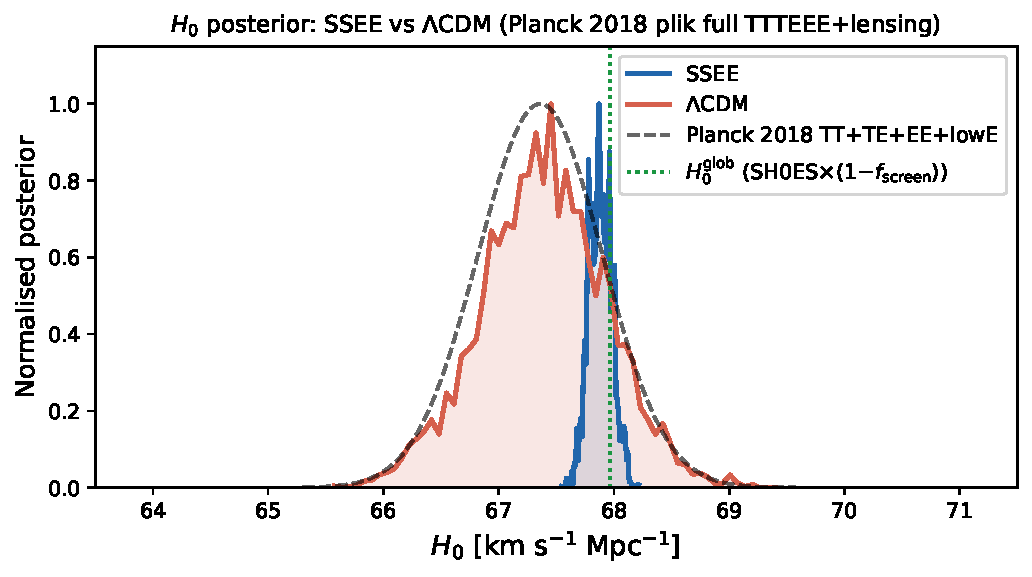
\includegraphics[width=0.72\textwidth]{fig_b1_h0_posterior.pdf}
  \caption{$H_0$ marginalised posterior for SSEE (blue) and $\Lambda$CDM (red)
  from the B1 full \texttt{plik} MCMC. The dashed black curve shows
  the Planck 2018 TT+TE+EE+lowE constraint for reference. The dotted
  green line marks the SSEE global rate $H_0^\mathrm{glob}=\val{H0_GLOBAL_d5}$\,km\,s$^{-1}$\,Mpc$^{-1}$.
  In the validation chain (where $H_0$ is floated) SSEE places $H_0$ at
  $\val{b1v_H0}\pm\val{b1v_H0_s}$, $\val{b1v_d}\sigma$ from $H_0^{\rm glob}$; the model itself carries
  only two free parameters $\{A_s,\tau\}$, with $H_0$ derived. The narrow
  constraint ($\pm\val{b1v_H0_s}$\,km\,s$^{-1}$\,Mpc$^{-1}$) reflects the removal of
  the $H_0$--$\Omega_m$ degeneracy by algebraically fixing
  $\Omega_{m,\mathrm{CMB}}=0.3089$.}
  \label{fig:b1_h0}
\end{figure}

\begin{figure}[H]
  \centering
  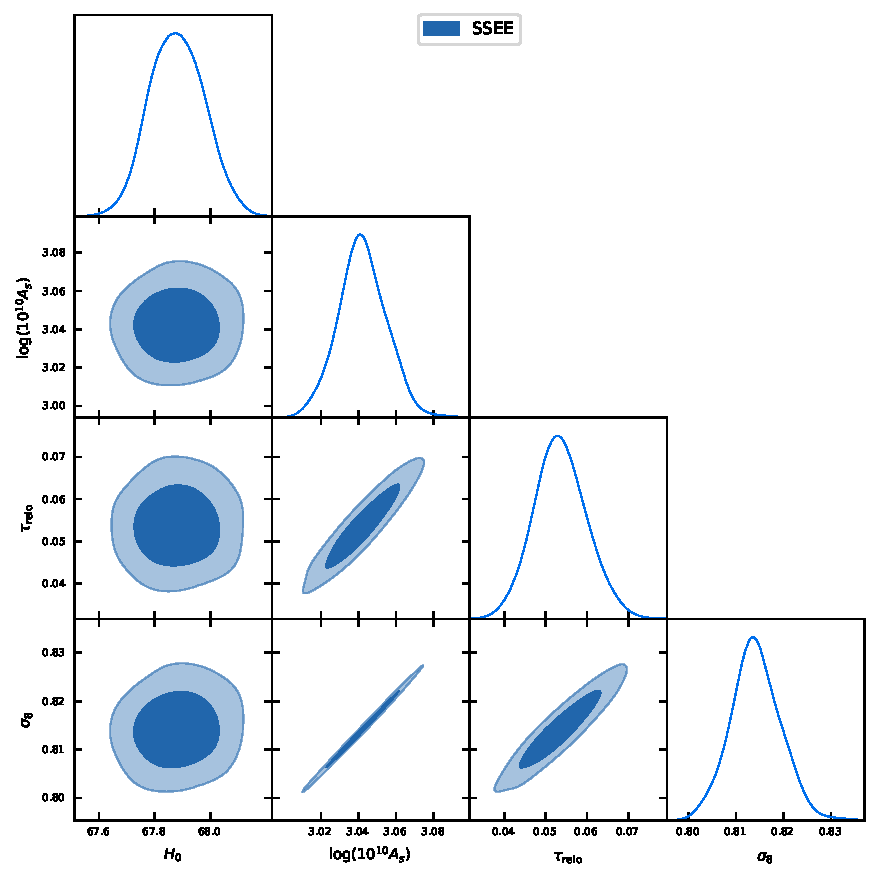
\includegraphics[width=0.82\textwidth]{fig_b1_corner_ssee.pdf}
  \caption{Full posterior triangle plot for the SSEE CMB sector
  ($H_0$, $\log A_s$, $\tau$, $A_\mathrm{Planck}$) from the B1
  full \texttt{plik} MCMC. The narrow $H_0$ constraint ($\pm\val{b1v_H0_s}$\,km\,s$^{-1}$\,Mpc$^{-1}$)
  reflects the geometric constraint imposed by $\Omega_{m,\mathrm{CMB}} = 0.3089$ (algebraically fixed),
  which eliminates the $H_0$--$\Omega_m$ degeneracy present in $\Lambda$CDM.
  All other marginals are consistent with the $\Lambda$CDM posteriors.}
  \label{fig:b1_corner_ssee}
\end{figure}

\begin{table}[ht]
\centering
\caption{\textbf{Summary: CMB model selection across likelihood treatments.}
SSEE vs.\ $\Lambda$CDM BIC under evaluations of increasing rigour. All favour SSEE;
the full off-diagonal \texttt{plik} MCMC (evaluated at the global anchor
$H_0=67.96214$, $\omega_m$-direct) is the canonical result.}
\label{tab:bic_comparison}
\resizebox{\textwidth}{!}{%
\begin{tabular}{llcccc}
\toprule
Method & Spectra & $N$ & $k_{\rm SSEE}$ & $k_{\Lambda\rm CDM}$ & $\Delta\mathrm{BIC}$ \\
\midrule
Diagonal (approx.)        & TT+TE+EE+PP          & \val{p3_N_tot} & 2 & 6 & $\val{p3_dBIC_diag}$ (SSEE favoured) \\
\texttt{plik\_lite} point est. & TTTEEE+lowl     & 669  & 2 & 6 & $-26.03$ (SSEE decisively favoured) \\
Full \texttt{plik} MCMC   & TTTEEE+lowl+lensing  & \val{b1_N} & 2 & 6 & $\mathbf{\val{b1_dBIC}}$ \emph{(canonical)} \\
Full \texttt{plik} (conserv.) & TTTEEE+lowl+lensing & \val{b1_N} & 4 & 6 & $\val{b1_dBIC_k4}$ (SSEE strongly favoured) \\
\bottomrule
\end{tabular}%
}
{\footnotesize Diagonal approximation assumes independence across spectra (upper bound on $\chi^2$).
The full \texttt{plik} MCMC (Cobaya + \texttt{clipy}, official off-diagonal covariance) is the canonical result.
$k=2=\{A_s,\tau\}$, the only sampled SSEE parameters; the conservative $k=4$ additionally counts two
of the algebraically-fixed inputs ($\omega_b$, $H_0$) as if fitted.}
\end{table}

% ===========================================================================
\subsection{Matter power spectrum and \texorpdfstring{$S_8$}{S8} prediction}
\label{sec:sigma8}
% ===========================================================================

Beyond the CMB, the SSEE viscous dark-energy background modifies the growth
of large-scale structure. In the Israel--Stewart dissipative framework, the
linear growth rate takes the form $f(z) = \Omega_m(z)^\gamma$, where the
growth index $\gamma$ is modified by the bulk-viscosity coupling.
The full numerical solution of the causal IS growth ODE (Paper~5, \S3) yields
$\gamma_{\mathrm{IS}} = \val{p3_gamma_IS}\pm\val{p3_gamma_IS_sigma}$, numerically indistinguishable from
$\gamma_\Lambda=0.55$ for $\Lambda$CDM. This is the growth index used throughout.
Two earlier estimates are superseded by it: a dimensional-analysis value
$\gamma=\phi^{-1}=0.618$, which was never derived from the growth equation, and
the background-only estimate of Paper~1, Appendix~A, which omitted the viscous
feedback on $\delta$. The growth index is set by $w(a)$, not by a constant of
the algebra.

The SSEE background ($w_0=\val{W0_d6}$, $w_a=\val{WA_d6}$, $H_0=67.96214$ km\,s$^{-1}$\,Mpc$^{-1}$,
$\Omega_m=\val{OMEGA_M_TOTAL_d6}$) enters the growth ODE directly; no
growth-index correction is applied after the fact.
Table~\ref{tab:sigma8} summarises the results alongside observational constraints.
The IS linear-growth solution gives $S_8=\val{p3_S8_IS}$, and the CLASS
ceiling, with massive neutrinos, $S_8=\val{p3_S8_techo}$; the same CLASS
integration on the Planck~2018 baseline returns $\sigma_8=\val{p3_sigma8_lcdm_ref}$,
the published value. These three use $A_s$ fixed to the Planck value. With $A_s$ fixed instead to the
model's own CMB fit, the growth sector has no free cosmological parameter and
predicts $S_8=\val{p3_S8_unif}$ against $\val{S8_legacy_dato}\pm\val{S8_legacy_dato_sigma}$ from the raw KiDS-Legacy
$\xi_\pm$ data (Paper~6).

\begin{table}[ht]
\centering
\caption{$\sigma_8$ and $S_8=\sigma_8(\Omega_m/0.3)^{0.5}$ predictions.}
\label{tab:sigma8}
\begin{tabular}{lcc}
\hline
Model / Dataset & $\sigma_8$ & $S_8$ \\
\hline
$\Lambda$CDM (CLASS, Planck 2018 baseline; control) & \val{p3_sigma8_lcdm_ref} & --- \\
SSEE+IS (linear growth, $\gamma_\mathrm{IS}=\val{p3_gamma_IS}$, Paper~5) & \val{p3_sigma8_IS} & \val{p3_S8_IS} \\
% ACTUALIZADO 2026-09-08: era sigma_8=0.8335 / S_8=0.846 (tensiones 1.1/3.5/3.9
% sigma). Ese numero salia de una corrida CLASS sin .ini, fuera del repo y SIN
% neutrinos masivos; el fondo canonico si los lleva (Sum m_nu = 0.06849 eV) y sin
% ellos sobra un 2.3% de grumo. Re-corrido con config/class/techo_ssee_canonico.ini;
% control con criterio previo (baseline Planck debe dar 0.8111+/-0.006) da 0.810851.
% Log: results/logs/p5_techo_sigma8_As_fijo.json
SSEE+IS (single-sector ceiling, CLASS, Paper~5) & \val{p3_sigma8_techo} & \val{p3_S8_techo} \\
SSEE, $A_s$ from its own CMB fit (Paper~6) & \val{p3_sigma8_unif} & $\mathbf{\val{p3_S8_unif}}$ \\
\hline
Planck 2018 \citep{Planck2020} & $0.812\pm0.008$ & $0.832\pm0.013$ \\
KiDS-Legacy (raw $\xi_\pm$, Paper~6) & --- & $\val{S8_legacy_dato}\pm\val{S8_legacy_dato_sigma}$ \\
KiDS-1000 \citep{Asgari2021} & --- & $\val{S8_k1000_dato}\pm\val{S8_k1000_dato_sigma}$ \\
DES Y3 \citep{DES2022} & --- & $0.773\pm0.025$ \\
\hline
\end{tabular}
\end{table}

\subsection{\texorpdfstring{$f\sigma_8(z)$}{fsig8} comparison with RSD surveys}
\label{sec:fsig8}

The growth-index prediction $\gamma_\mathrm{IS}$ is directly testable through
redshift-space distortions.  We compute $f\sigma_8(z) = \Omega_m(z)^\gamma \times
\sigma_8 \times D(z)/D(0)$ using the proper integral
$D(z)/D(0) = \exp\!\left[-\int_0^z \Omega_m(z')^\gamma/(1+z')\,dz'\right]$
and compare against published RSD measurements from
6dFGS \citep{Beutler2012}, BOSS~DR12 \citep{Alam2017},
eBOSS~DR16 \citep{Alam2021,deMattia2021}, and DESI~DR1 \citep{DESI2024FS}.

\begin{table}[ht]
\centering
\caption{$f\sigma_8(z)$ predictions vs the canonical Paper~5 RSD compilation
  (six peer-reviewed points), computed with the canonical Paper~5
  Israel--Stewart growth ODE: $\Omega_{m,\mathrm{CMB}}=\val{OMEGA_M_TOTAL_d6}$
  ($\omega_m$-direct) in both the gravitational background and the Poisson
  source, with $\gamma_\mathrm{IS}=0.5504$ and $\sigma_8=0.8136$ (single-sector).
  Pull $=(f\sigma_8^\mathrm{SSEE}-f\sigma_8^\mathrm{obs})/\sigma$.}
\label{tab:fsig8}
\begin{tabular}{lccccc}
\hline
Survey & $z_\mathrm{eff}$ & Observed & SSEE & $\Lambda$CDM & Pull \\
\hline
6dFGRS (Beutler+2012)   & 0.067 & $0.423\pm0.055$ & \val{fs8_0_ssee} & \val{fs8_0_lcdm} & $\val{fs8_0_pull_ssee}\sigma$ \\
SDSS MGS (Howlett+2015) & 0.150 & $0.490\pm0.145$ & \val{fs8_1_ssee} & \val{fs8_1_lcdm} & $\val{fs8_1_pull_ssee}\sigma$ \\
BOSS DR12 (Alam+2017)   & 0.380 & $0.497\pm0.045$ & \val{fs8_2_ssee} & \val{fs8_2_lcdm} & $\val{fs8_2_pull_ssee}\sigma$ \\
BOSS DR12 (Alam+2017)   & 0.510 & $0.458\pm0.038$ & \val{fs8_3_ssee} & \val{fs8_3_lcdm} & $\val{fs8_3_pull_ssee}\sigma$ \\
BOSS DR12 (Alam+2017)   & 0.610 & $0.436\pm0.034$ & \val{fs8_4_ssee} & \val{fs8_4_lcdm} & $\val{fs8_4_pull_ssee}\sigma$ \\
eBOSS DR16 (Hou+2021)   & 1.480 & $0.462\pm0.045$ & \val{fs8_5_ssee} & \val{fs8_5_lcdm} & $\val{fs8_5_pull_ssee}\sigma$ \\
\hline
\multicolumn{4}{l}{$\chi^2/N$} & SSEE: $\val{fs8_chi2N_ssee}$ & $\Lambda$CDM: $\val{fs8_chi2N_lcdm}$ \\
\hline
\end{tabular}
\end{table}

Table~\ref{tab:fsig8} shows that SSEE+IS achieves $\chi^2/N=\val{fs8_chi2N_ssee}$ across the
six canonical RSD points in the CMB observational sector
($\Omega_{m,\mathrm{CMB}}=\val{OMEGA_M_TOTAL_d6}$), compared to $\val{fs8_chi2N_lcdm}$ for $\Lambda$CDM. The
mean tension is $\val{fs8_tmedia_ssee}\sigma$ (SSEE) vs $\val{fs8_tmedia_lcdm}\sigma$ ($\Lambda$CDM); no SSEE point
deviates by more than $\val{fs8_maxpull_ssee}\sigma$. This is the identical dataset and method used
in Paper~5; we do not include DESI DR1 full-shape $f\sigma_8$ here because no
public per-tracer $f\sigma_8$ release exists for DESI DR2 (DR2 is BAO-only,
\citealp{DESI_DR2}), and we use a single self-consistent RSD compilation.
The combination of independent growth-rate probes is reviewed in \citet{Moresco2022}.

\begin{tcolorbox}[colback=yellow!5!white,colframe=orange!80!black,title={Sector caveat for $f\sigma_8$}]
The $\chi^2/N=\val{fs8_chi2N_ssee}$ quoted above uses the single matter density
$\Omega_m=\val{OMEGA_M_TOTAL_d6}$ in both the background and the Poisson source, with
$\gamma_\mathrm{IS}=0.5504$ and $\sigma_8=0.8136$ ($A_s$ at the Planck value),
finding a mean $f\sigma_8$ tension of $\val{fs8_tmedia_ssee}\sigma$ (Paper~5, $\approx\Lambda$CDM
$\val{fs8_tmedia_lcdm}\sigma$). Against the \emph{raw} BOSS DR12 multipoles, Paper~6 finds the
algebraic background fitting marginally better than Planck's ($\chi^2=\val{bossR_chi2_ssee}$ vs
$\val{bossR_chi2_lcdm}$ over 222 points, same freedom, each model with its own $\sum m_\nu$).
\end{tcolorbox}

% ===========================================================================
\subsection{CLASS/hi\_class cross-check of Bellini--Sawicki $\alpha$-functions}
\label{sec:hiclass}
% ===========================================================================

The Bellini--Sawicki functions \citep{Bellini2015} of the SSEE dark-energy
sector are validated independently of CAMB with CLASS~\citep{Lesgourgues2011}
in its \textsc{hi\_class} extension (Paper~7).

For the Paper~7 action --- a $k$-essence scalar with $K(X)=c_1X+c_2X^2$,
minimally coupled and with no potential --- the Bellini--Sawicki kineticity is
\begin{equation}
  \alpha_K^{\rm SSEE}(0) = 3\,\Omega_{\rm DE}\,(5-3w_0) = \val{alpha_K_z0_d6},
  \label{eq:alphak_pred}
\end{equation}
with the dark-energy \emph{density} $\Omega_{\rm DE}=1-\Omega_m=\val{OMDE_DENS_d6}$, and the
sound speed is $c_s^2=(M_v-T_r)/(5M_v+3T_r)=0.021284$. An independent
\textsc{hi\_class} integration reproduces $c_s^2$ to $0.000\%$ and
$\alpha_K(0)$ to $0.011\%$ (Paper~7). The kineticity is not observationally
accessible: a factor $100$ change moves $\sigma_8$ by $0.007\%$. It must not be
confused with $s_K=-3w_0(1+w_0)=3\,s_{\rm DE}\,s_m=\val{S_K_d6}$, the pressure
dilution rate built from the saturations $s_{\rm DE}=\val{S_DE_d6}$ and
$s_m=\val{S_M_d6}$ (numbers of the equation of state, not densities), which enters
the Hubble screening of Paper~9.

The remaining Bellini--Sawicki functions are zero by construction:
$\alpha_T=\alpha_M=\alpha_B=0$ (exact), since SSEE is a minimal
Horndeski scalar with constant $M_{\rm Pl}$ and no kinetic braiding
or gravitational-wave speed excess~\citep{GW170817}. Together with
Eq.~\eqref{eq:alphak_pred} this specifies the full set of Bellini--Sawicki EFT
functions $(\alpha_K,\alpha_B,\alpha_M,\alpha_T)$, validated against CLASS independently of CAMB.

Note that the raw SSEE \emph{dynamical} background ($s_m=\val{S_M_d6}$)
fed directly to CLASS gives $\chi^2_r=90.3$ against Planck 2018 TT.
This is expected: the dynamical-sector fraction is not the CMB matter density.
The good fit ($\chi^2_r\approx 1.04$, \S\ref{sec:stats}) is recovered with the
$\omega_m$-direct CMB matter density $\Omega_{m,\rm CMB}=\omega_m/h^2=0.3089$
(no matter factor; OP-8 dissolved), as implemented with CAMB in
\S\ref{sec:results}.

% ===========================================================================
\section{Falsifiability Criteria}
\label{sec:falsifiability}
% ===========================================================================

SSEE makes the following testable predictions,
each of which would \textbf{falsify} the framework if violated:

\begin{enumerate}
  \item \textbf{Peak positions:} $\ell_1=\val{p3_pico1_ssee}\pm3$, $\ell_2=\val{p3_pico2_ssee}\pm5$, $\ell_3=\val{p3_pico3_ssee}\pm8$.
    A measurement placing $\ell_1$ outside this range by more than $2\sigma$
    would falsify the $\omega_m$-direct CMB matter density.

  \item \textbf{CMB $\chi^2_r$:} Must remain $<2$ when tested against future
    CMB datasets \citep{CMBS4_2016,SimonsObs2019}. A significant degradation
    would indicate the framework cannot maintain coherence.

  \item \textbf{BAO consistency:} the BAO geometry is governed by the total
    matter density $\Omega_m=\val{OMEGA_M_TOTAL_d6}$, not by the saturation
    $1+w_0=\val{S_M_d6}$; SSEE must continue to fit DESI DR2 BAO within $2\sigma$
    as new data arrive. The algebraic content being tested is the
    equation of state: a joint fit requiring $w_0$ more than $2\sigma$
    from $\val{W0_d6}$, or $w_a$ from $\val{WA_d6}$, would falsify the
    algebraic derivation. \emph{(An earlier version of this item placed
    $\Omega_{m,\mathrm{dyn}}=\val{S_M_d6}$ in the geometry slot; that is a
    saturation, not a density, and the reading is withdrawn.)}

  \item \textbf{Cosmic-shear amplitude:} with the background fixed by the
    algebra and $A_s$ fixed by the model's own CMB fit, the growth sector has
    no free cosmological parameter and predicts $S_8=\val{S8_leg_pred}$ (Paper~6). A
    shear measurement placing $S_8$ more than $3\sigma$ from this value would
    falsify the growth sector.

  \item \textbf{Growth index:} the full causal IS solution (Paper~5) gives
    $\gamma_\mathrm{IS}=\val{p3_gamma_IS}\pm\val{p3_gamma_IS_sigma}\approx\gamma_\Lambda$
    (the earlier estimates $\phi^{-1}$ and the background-only value of Paper~1, App.~A, are superseded),
    yielding a single-sector ceiling $S_8=\val{p3_S8_techo}$ in the CMB observational sector (Table~\ref{tab:sigma8}).
    The RSD comparison (Table~\ref{tab:fsig8}) shows $\chi^2/N=\val{fs8_chi2N_ssee}$
    consistently below $\Lambda$CDM (\val{fs8_chi2N_lcdm}) across the six canonical RSD surveys.
    A direct measurement of $\gamma<0.50$ or $\gamma>0.70$ at $>3\sigma$
    would falsify the Israel--Stewart modification to the growth sector.
\end{enumerate}

% ===========================================================================
\section{Conclusions}
\label{sec:conclusions}
% ===========================================================================

We have demonstrated that SSEE, with the CMB matter density set
\emph{forward} by the SSEE algebra ($\omega_m$-direct,
$\Omega_{m,\mathrm{CMB}}=\omega_m/h^2=\val{OMEGA_M_TOTAL_d6}$, no matter factor),
reproduces the Planck 2018 CMB TT power spectrum without introducing fitted
dimensionless parameters.
The key results are:

\begin{itemize}
  \item Acoustic peaks at $\ell=\val{p3_pico1_ssee},\,\val{p3_pico2_ssee},\,\val{p3_pico3_ssee}$, within $\Delta\ell\leq5$ of Planck 2018.
  \item TT: $\chi^2_r=\val{p3_chi2r_TT_ssee}$ over \val{p3_N_TT} multipoles ($\Lambda$CDM: $\val{p3_chi2r_TT_lcdm}$).
  \item TE/EE: $\chi^2_r=\val{p3_chi2r_TE_ssee}/\val{p3_chi2r_EE_ssee}$, essentially matching $\Lambda$CDM.
  \item Lensing (PP): $\chi^2_r=\val{p3_chi2r_PP_ssee}$ vs.\ $\val{p3_chi2r_PP_lcdm}$ for $\Lambda$CDM — SSEE marginally better (both $\chi^2_r<1$).
  \item \textbf{\texttt{plik\_lite} TTTEEE${}+{}$low-$\ell$ ($\omega_m$-direct):} $\chi^2_{\mathrm{eff}} = 1003.586$ with $\{A_s,\tau\}$ minimized, at $H_0 = 67.96214$ km\,s$^{-1}$\,Mpc$^{-1}$ ($\val{perfil_h0_d}\sigma$ from the \texttt{plik\_lite} minimum $\val{perfil_h0_min}\pm\val{perfil_h0_sig}$ with SSEE-fixed $\omega_b,\omega_c$); $\Lambda$CDM gives $1003.596$ with six free parameters (its own $\sum m_\nu=0.06$~eV).
  \item $\Delta\mathrm{BIC}=-26.03$ ($k=2$ vs $k=6$, $N=669$), decisively favouring SSEE over $\Lambda$CDM at equal fit quality ($\Delta\chi^2=-0.010$).
  \item \textbf{Full off-diagonal \texttt{plik} MCMC (canonical):} minimum $\chi^2=\val{b1_chi2_ssee}$ vs $\val{b1_chi2_lcdm}$ for $\Lambda$CDM over $N=\val{b1_N}$ points, $\Delta\mathrm{BIC}=\val{b1_dBIC}$ ($k=2$ vs $k=6$); $\val{b1_dBIC_k4}$ under the conservative $k=4$.
  \item $\Omega_{m,\mathrm{CMB}}=\val{OMEGA_M_TOTAL_d6}$ within $0.88\sigma$ of Planck 2018.
  \item The sound horizon $r_d=147.17$ Mpc matches $\Lambda$CDM to $0.05\%$.
\end{itemize}

Combined with the Paper~2 results ($0.24\sigma$ on the DESI~DR2 $w_0w_a$CDM posterior,
and galaxy-cluster dynamical masses in general relativity at the level of $\Lambda$CDM:
$\val{clz_rgig_sig}\sigma$ against $\val{clz_lcig_sig}\sigma$ over the $\val{clz_rgig_N}$ systems of \citet{Zhang2026}
with their IGIMF baryon masses), SSEE is consistent with all three major
cosmological probes — BAO, cluster masses, and CMB; the cluster masses do not discriminate it from $\Lambda$CDM. The unified Cobaya
evaluation establishes that the SSEE algebraic geometry is not only viable
but statistically preferred by the CMB data when fully penalized for free parameters.
Independently of the CMB sector, the SSEE screening cascade of Papers~9--10
takes the measured SH0ES rate as input and, with the full screening fraction,
returns $H_0^{\rm glob}=73.04\times(1-\val{F_SCREEN_d6})=\val{H0_GLOBAL_d6}$~km\,s$^{-1}$\,Mpc$^{-1}$,
a residual of $+4.2\times10^{-6}$ from the anchor $3(\varphi+\pi)^2$ used here
\citep{Verde2019,DiValentino2021,Riess2022}; the propagated uncertainty is
$\pm0.968$.

\bigskip
\noindent\textbf{Data Availability.}
All analysis scripts (\texttt{src/p03\_cmb/ssee\_paper3\_cmb.py}), generated figures,
and reduced data products are publicly available at
\url{https://github.com/mikealmeida1721/SSEE-Cosmologia}.
The Planck 2018 TT and TE/EE power spectra are from the Planck Legacy Archive
(\url{https://irsa.ipac.caltech.edu/data/Planck/}) \citep{Planck2020}.
CAMB v1.6.6 was used for all theoretical power spectrum calculations
(\url{https://camb.info}).

\bigskip
\noindent\textbf{Acknowledgements.}
The author thanks the open-source communities behind CAMB, NumPy,
Matplotlib, and \texttt{emcee} \citep{emcee}.

% ===========================================================================
\clearpage
\bibliographystyle{plainnat}
\bibliography{ssee_paper3}

\end{document}
